% don't remove the folling lines, and edit the defintion of \main if needed
\documentclass[../report.tex]{subfiles}
\providecommand{\main}{..}
\IfEq{\jobname}{\currfilebase}{\AtEndDocument{\biblio}}{}
% until here

%\newcommand{\mlna}{\langle \ln\!A \rangle}
%\newcommand{\nmu}{N_\mu}
%\newcommand{\lnnmu}{\ln\!\nmu}
%\newcommand{\xmax}{X_\text{max}}
%\newcommand{\nmult}{N_\text{mult}}
%\newcommand{\tocite}{{\bf REF}}
%\newcommand{\si}[1]{\ensuremath{\text{#1}}}
%\newcommand{\SI}[2]{\ensuremath{#1\,\si{#2}}}

%\newcommand{\pt}{p_\mathrm{T}}

\begin{document}

\section{Other opportunities with ion and proton beams at the LHC}
%%%%%%%%%%%%%%%%%%%%%%%%%%%%%%%%%%%%%%%%%%%%%%%%%%%%%%%%%%%%%%%%%%%%%%
\subsection{Physics motivation for collisions of light ions}
\label{sec:smallAsum}
{ \small
\noindent \textbf{Coordinator}: Z. Citron (Ben-Gurion University of the Negev)

\noindent \textbf{Contributors}:
L. Apolinario (LIP and IST Lisbon),
C. Loizides (Oak Ridge National Laboratory),
G. Milhano (LIP and IST Lisbon, CERN),
A. Milov (Weizmann Institute of Science),
A. Sickles (U. Illinois, Urbana-Champaign)
}

The collision of ion species with A$\ll$A$_\mathrm{Pb}$ is an appealing opportunity to expand the physics programme presented in this document.  The recent \XeXe run of only eight hours has provided valuable input for the physics performance of ion collisions lighter than Pb at the LHC.  Broadly, the advantages of using A$\ll$A$_\mathrm{Pb}$  collisions are twofold: smaller collision systems sample key physical parameters beyond what can be probed with \PbPb and \pPb collisions, and they allow higher luminosity running to maximize the accumulation of rare events in heavy-ion collisions.  This higher luminosity could enable a high-precision paradigm for currently rare observables in \PbPb collisions as well as the study of observables totally inaccessible in \PbPb collisions.        
A two-pronged scenario is envisioned composed of a short run of \OO  ($A=16$) and longer running of a species of intermediate A.  The choice of the intermediate species will be dictated by the competition of increased luminosity with lower A against the goal of studying the properties of an extended QGP system. Optimizing the choice of species will require further study from the accelerator, experimental, and theoretical communities; in this document \ArAr ($A=40$) collisions are considered as a test-case for the choice of intermediate ion.

Section \ref{sec:lightions} describes the technical capabilities of the LHC to provide lighter-ion collisions, as well as describing the expected performance for several different ion species.
For example, for \ArAr the expectation for one month of collisions is 1080 $\invnb$ ($p$=1.5).  In order to compare across different collisions species we consider the \textit{nucleon--nucleon} integrated luminosity per month of running, which could be larger by a factor 3--23 (for $p$=1.2--1.9) with respect to \PbPb collisions, \textit{i.e.} one month of \ArAr collisions would be equivalent to 25--80 $\invnb$ of \PbPb collisions. This gain would be the same in all centrality classes (defined in terms of percentiles of the hadronic cross section).
Section \ref{sec:flow_sizedep} discusses flow measurements possible using smaller species.  A discussion of the role light ion collisions can play for low-$x$ and nPDF studies is found in sect.~\ref{sec:nPDF_lightions}.  The implications of \ArAr collisions for the study of light-by-light scattering are discussed in Sect.~\ref{sec:upc}. 

Even a short \OO run can help clarify the uncertainty concerning the onset of QGP or QGP-like phenomena in high-multiplicity pA and pp collisions discussed in section \ref{sect:smallsystems_OO}.  The search for basic properties associated with the QGP in \OO collisions should complement the searches in \pp and \pPb collisions.% systems, \textit{i.e.} if they can not be observed in \OO there should be no reasonable expectation of observing them in smaller collisions systems.  
In particular, the \OO system has well-understood collision geometry as described in detail in Sect.~\ref{sect:smallsystems_OO}, enabling the study of collisions with low values of $\langle N_{\rm part}\rangle$ that are difficult to select and study in \PbPb collisions and that are similar to those estimated for high-multiplicity \pPb events. Colliding \OO at the LHC naturally dovetails with \pO collisions whose significance for the cosmic-ray community is detailed in section \ref{sec:pOcosmic}.

Complementing \PbPb collisions, 
the possibility of high-luminosity extended LHC runs with intermediate-A nuclei (e.g.\ArAr)
is a promising long-term option.
%In addition to being a new system and thereby providing another data-point for observables that probe different geometries (see \textit{e.g.} Sect.~\ref{sec:flow_sizedep}),
The chief promise of \ArAr collisions is the possibility of reaching much higher luminosity than \PbPb collisions while still producing a QGP over an extended volume of $\sim 1000$~fm$^3$ in central events. Based on an MC Glauber simulation \cite{Loizides:2017ack}, the mean number of participants expected, $\langle N_{\rm part}\rangle$, for \ArAr ranges from  $\sim 7$ for 60--80\% centrality to $\sim 70$ for 0--5\% centrality collisions.  
QGP effects are observed in \PbPb collisions with similar number of participants \cite{Sirunyan:2018eqi, ATLAS-CONF-2018-007}.  In addition, the much lower underlying event multiplicity in \ArAr relative to central \PbPb collisions is expected to lead to reduced  systematic uncertainties for several observables, from reconstructed jets to all signal affected by large combinatorial backgrounds.  These features, combined with the possibility to increase the nucleon--nucleon luminosity by more than one order of magnitude, make \ArAr collisions an extremely attractive option for hard probe measurements that in \PbPb collisions are `statistics starved' or impossible, such as top quarks for QGP studies as outlined in \cite{Apolinario:2017sob}.  Figure \ref{fig:boosted_tops} extends the analysis to lighter nuclei and shows that one month of \ArAr collisions, with nucleon--nucleon luminosity equivalent to 25--80~$\invnb$ for \PbPb, allows a similar physics reach as the entire \PbPb future programme ($13~\invnb$), namely to probe the QGP density evolution up to a time of about 1.5--2~fm/$c$.  Top quark studies in \ArAr collisions in the context of constraints on nPDFs are detailed in section \ref{sec:nPDF_top}.
\begin{figure}
\centering
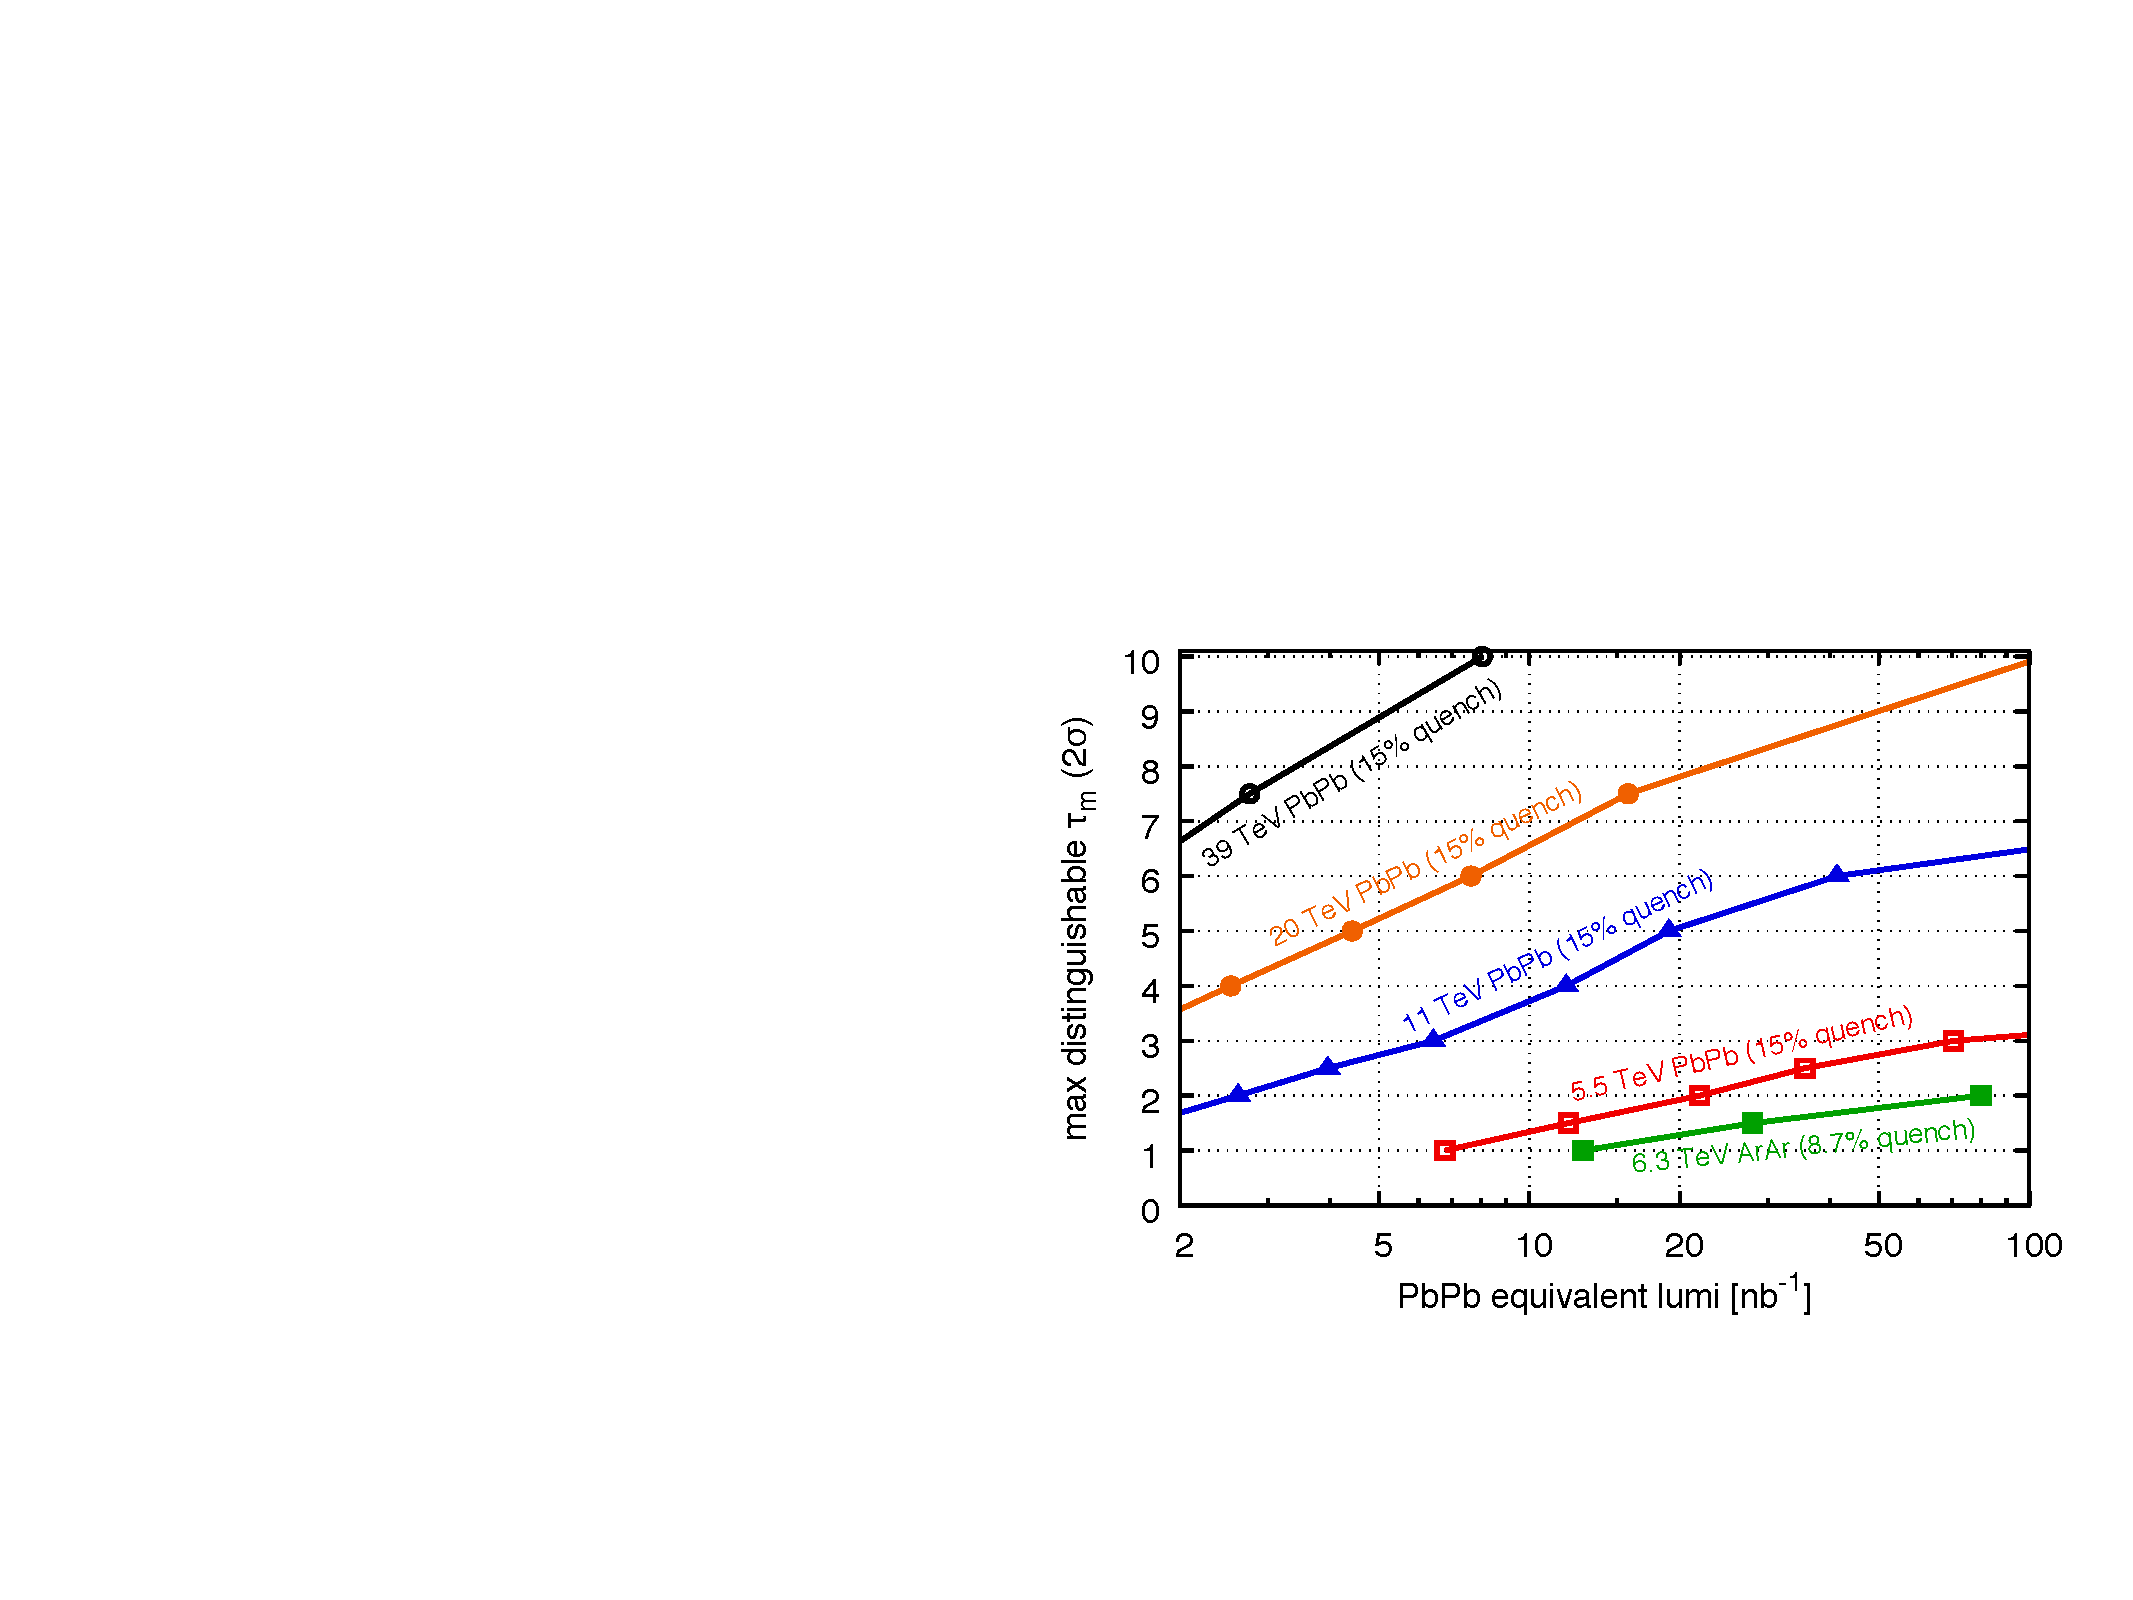
\includegraphics[width=0.68\linewidth]{\main/smallAexec/fig/top_plot}
\caption{Maximum medium lifetime that can be distinguished from a full quenching baseline with two standard deviations (2 $\sigma$), as a function of luminosity for different species and collider energies. The luminosity on the $x$-axis is maintaining an equal number of nucleon-nucleon collisions. A single \ArAr run is expected to provide $\sim$ 25--75 $\invnb$ of \PbPb equivalent luminosity.}
\label{fig:boosted_tops}
\end{figure}

Studies with $Z$ bosons are representative examples of the types of measurements that may be undertaken in a lighter ion rare-probes programme.  In Figure \ref{fig:Zreach} the expected number of $Z$ boson candidates (assuming a selection similar to that used by ATLAS and CMS in previous studies) for one month of heavy ion running  as a function of $\langle N_{\rm part}\rangle$ is shown for several different lighter ion species, and compared with the expectation for the full \PbPb and \pPb programmes.  The figure demonstrates that the overall yield of $Z$ bosons would be considerably higher for one \ArAr run than for several years of \PbPb running including both a sufficient number of candidates to study low $\langle N_{\rm part}\rangle$ collisions unreachable with \PbPb collisions as well as moderate $\langle\Npart\rangle$ values in which QGP formation is expected.  $Z$ bosons are a powerful tool to probe the properties of the QGP in particular in $Z$+jet events.  
\begin{figure}
\centering
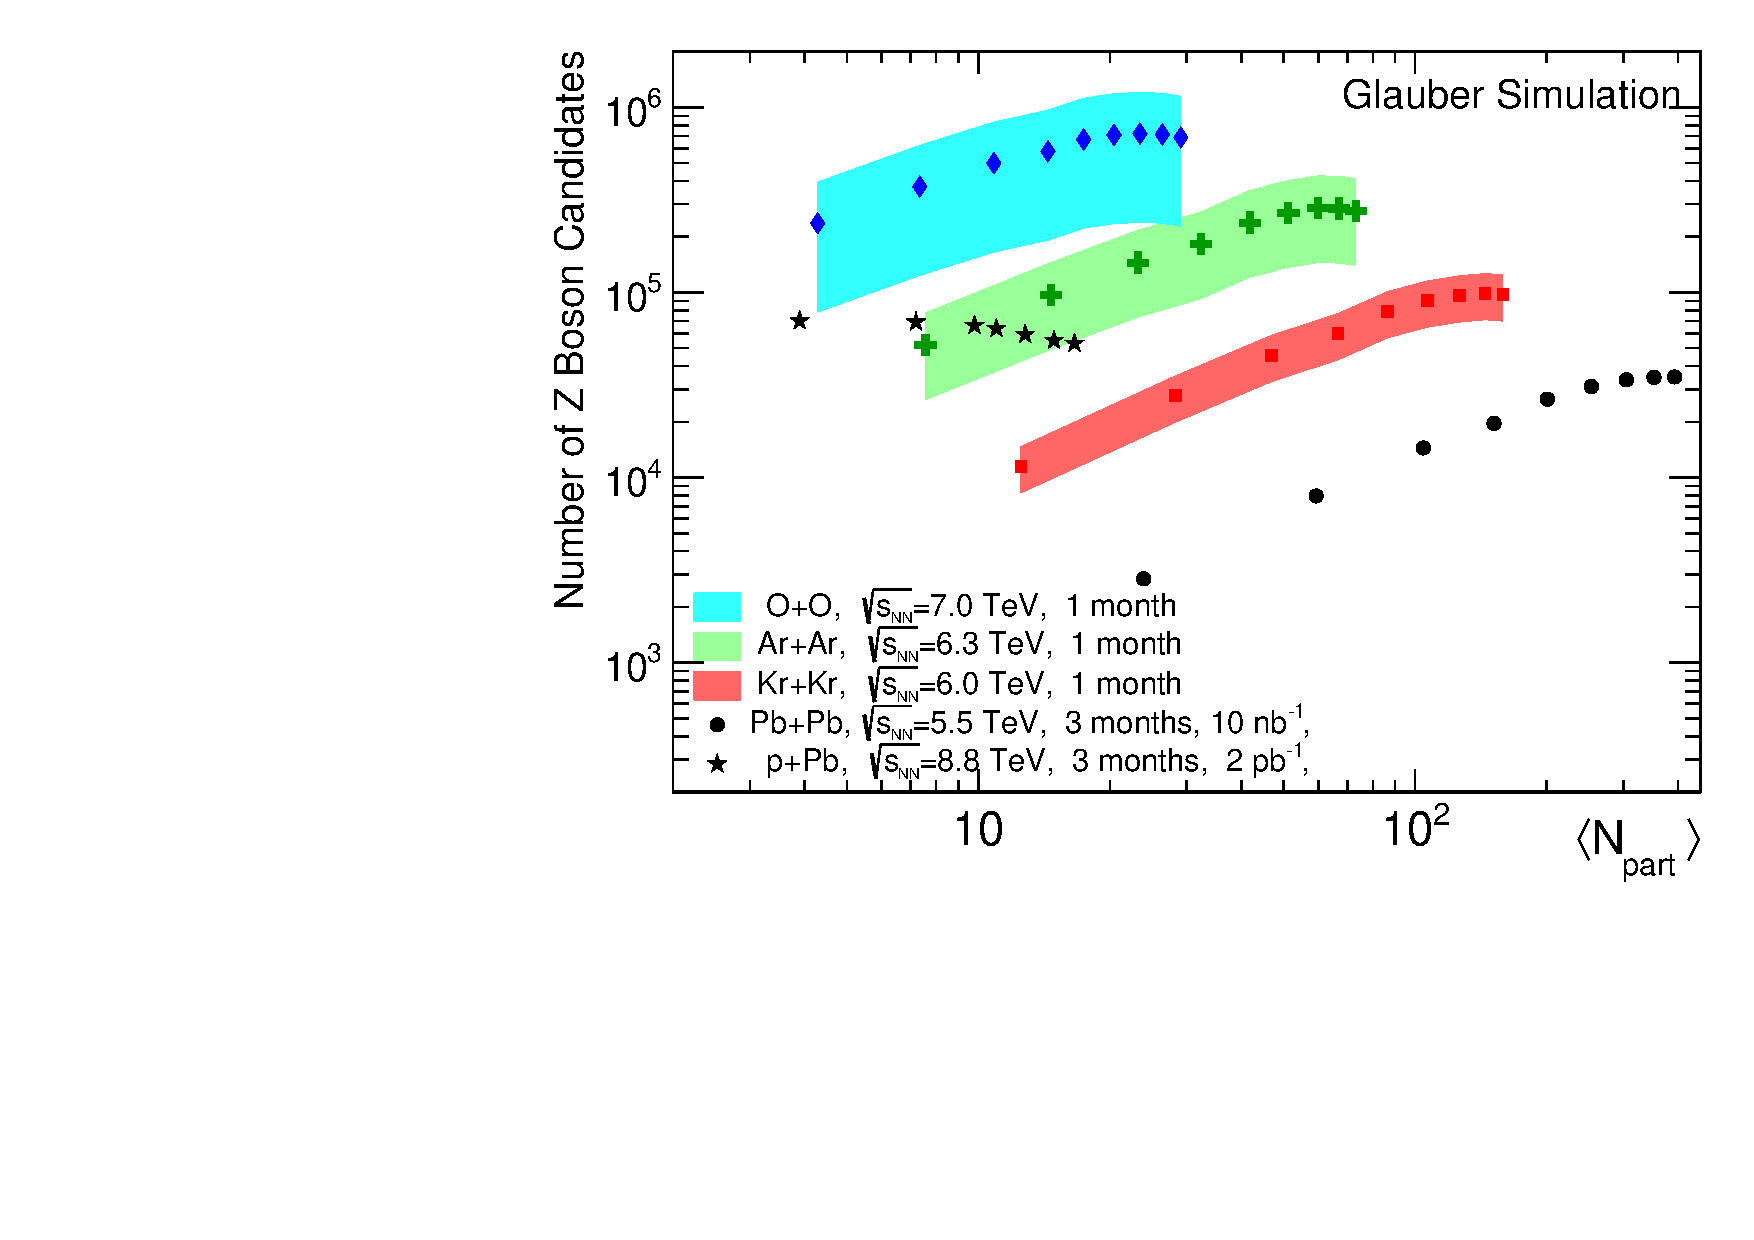
\includegraphics[width=0.68\linewidth]{\main/smallAexec/fig/Zcentreach}
\caption{
The number of $Z$ bosons as a function of $\langle N_{\rm part}\rangle$ expected for one full heavy-ion run at the LHC for several collisions species.  The $Z$ bosons are reconstructed via the di-lepton decay channel with leptonic $\pT>20$~GeV$/c$ and $|\eta|<2.5$, and a mass selection of $66<M_{\ell\ell}<116$~GeV.  Luminosities shown for \PbPb and \pPb correspond to several years of running.  The central values correspond to $p=1.5$ as discussed in section \ref{sec:lightions}, with the uncertainties representing a variation of $p$ down to 1 and up to 1.9.
\label{fig:Zreach}}
\end{figure}

$Z$+jet events were simulated in the 10\% most central events in \ArAr collisions using JEWEL \cite{Zapp:2009ud} to estimate the expected jet-quenching effects.  Figure \ref{fig:ArAr_xjz} shows the distribution of $x_{jZ}$, the ratio of the jet transverse momentum to that of the $Z$ boson for 0--10\% centrality \ArAr events, as well as \pp collisions and 0--10\% centrality \PbPb events ($N_{\rm part} = 356$, $T=360$ MeV at thermalization time $\tau = 0.55$ fm/$c$ for $\sqrt{s}=5.5$ TeV).  The $Z$ boson must have \pt $>$ 60 GeV/$c$ and be back-to-back ($\Delta\varphi > 7/8\pi$) to a jet with \pt $>$ 30 GeV/$c$.  The Figure clearly shows that for this observable the jet-quenching phenomena observed in \PbPb collisions as modelled by JEWEL are present also in \ArAr collisions.  This demonstrates the potential of the \ArAr (or a similar) collision system for a heavy ion rare probes programme.% with a much larger dataset than the LHC \PbPb program.
\begin{figure}
\centering
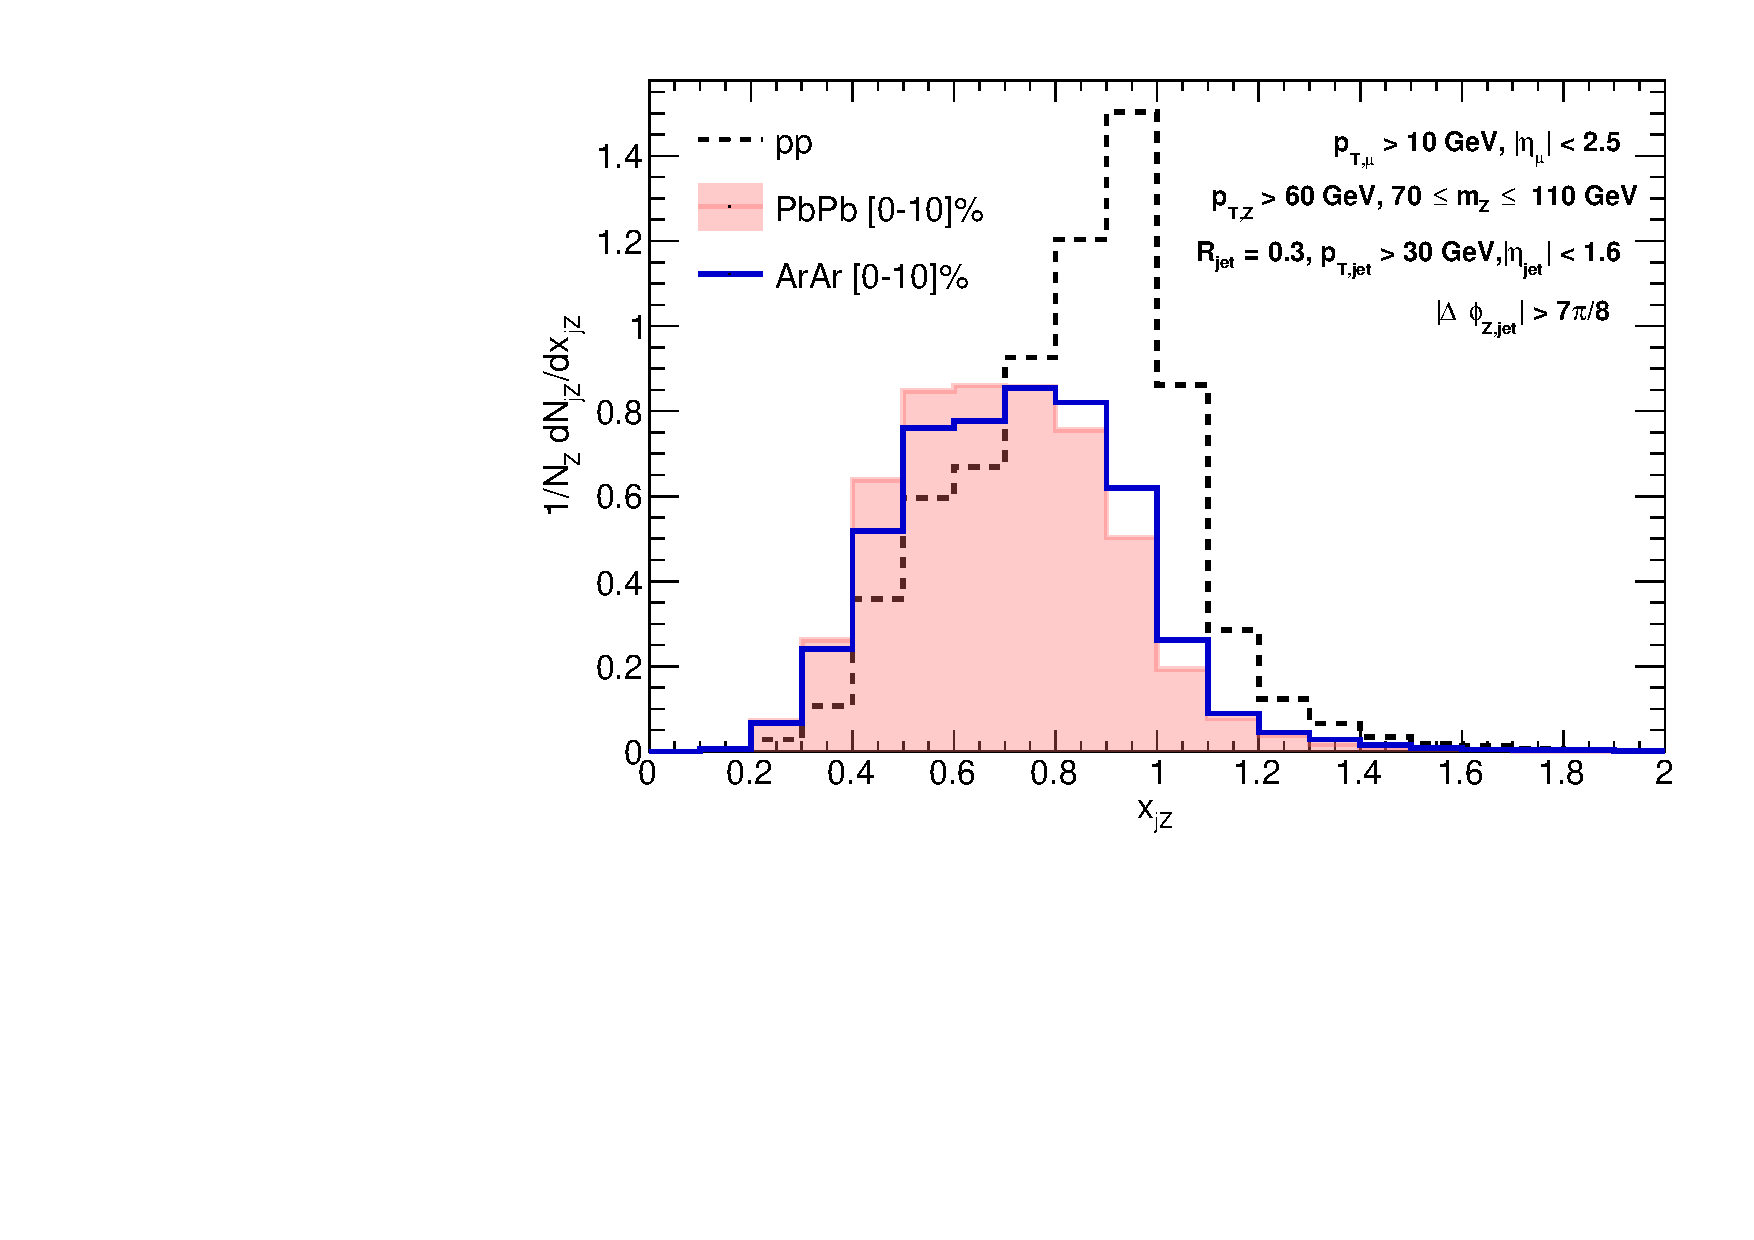
\includegraphics[width=0.48\linewidth]{\main/smallAexec/fig/Zjetassym}
\caption{
The $x_{jZ}$ distribution for pp, \PbPb, and \ArAr collisions calculated with JEWEL.  The 10\% most central events are shown for \PbPb and \ArAr.  \ArAr collisions are calculated as $N_{\rm part} = 60$, $T=318$ MeV at thermalization time $\tau = 0.63$ fm/$c$ for $\sqrt{s}=6.3$ TeV.  The $Z$ boson must have $\pt > 60$~GeV/$c$ and be back-to-back ($\Delta\varphi > 7/8\pi$) to a jet with $\pt > 30$~GeV/$c$.    
\label{fig:ArAr_xjz}}
\end{figure}

\clearpage
%%%%%%%%%%%%%%%%%%%%%%%%%%%%%%%%%%%%%%%%%%%%%%%%%%%%

\subsection{Physics of $\mathrm{\gamma \gamma}$ interactions in heavy-ion collisions}
\label{sec:upc}
%%%%%%%%%%%%%%%%%%%%%%%%%%%%%%%%%%%%%%%%%%%%%%%%%%%%%%%%%%%%%%%%%%%%%%

{ \small
\noindent \textbf{Coordinators}: Iwona Grabowska-Bold (AGH UST, Krak\'ow)\\

\noindent \textbf{Contributors}: 
M.~Dyndal (DESY), 
S.~Hassani (Universit\'e Paris-Saclay), 
M.~Klusek-Gawenda (IFJ PAN, PL-31342 Krak\'ow, Poland), 
L.~Schoeffel (Universit\'e Paris-Saclay), Peter Steinberg (BNL)
}

Heavy-ion beams are composed of nuclei which carry electric charge $Ze$~($e$ is the electron charge and $Z$ is the atomic number). They are accelerated to nearly the speed of light, thus they generate large electromagnetic~(EM) fields. 
The EM fields generated by the relativistic ion can interact with the other nucleus or its EM fields.
Therefore, besides nuclear hadronic interactions, EM
interactions also occur in ultra-relativistic heavy-ion collisions.
These EM interactions can be studied in so-called ultra-peripheral
collisions~(UPC) which occur when the distance between two nuclei in the transverse plane is larger than two times the nuclear radius, and hadronic interactions are thus suppressed~\cite{Bertulani:2005ru}.

A broad range of processes can be studied with $\mathrm{\gamma\gamma}$ interactions in UPC. In the following, a few examples of photon-induced processes are considered at the HL-LHC: exclusive production of $\mathrm{\mu^+\mu^-}$ or p$\mathrm{\bar{p}}$ pairs, a rare process of light-by-light~(LbyL) scattering and a potential of searches for axion-like particles~(ALP).

%-------------------------------------------------------------------
\begin{figure}[!hbt]
\centering
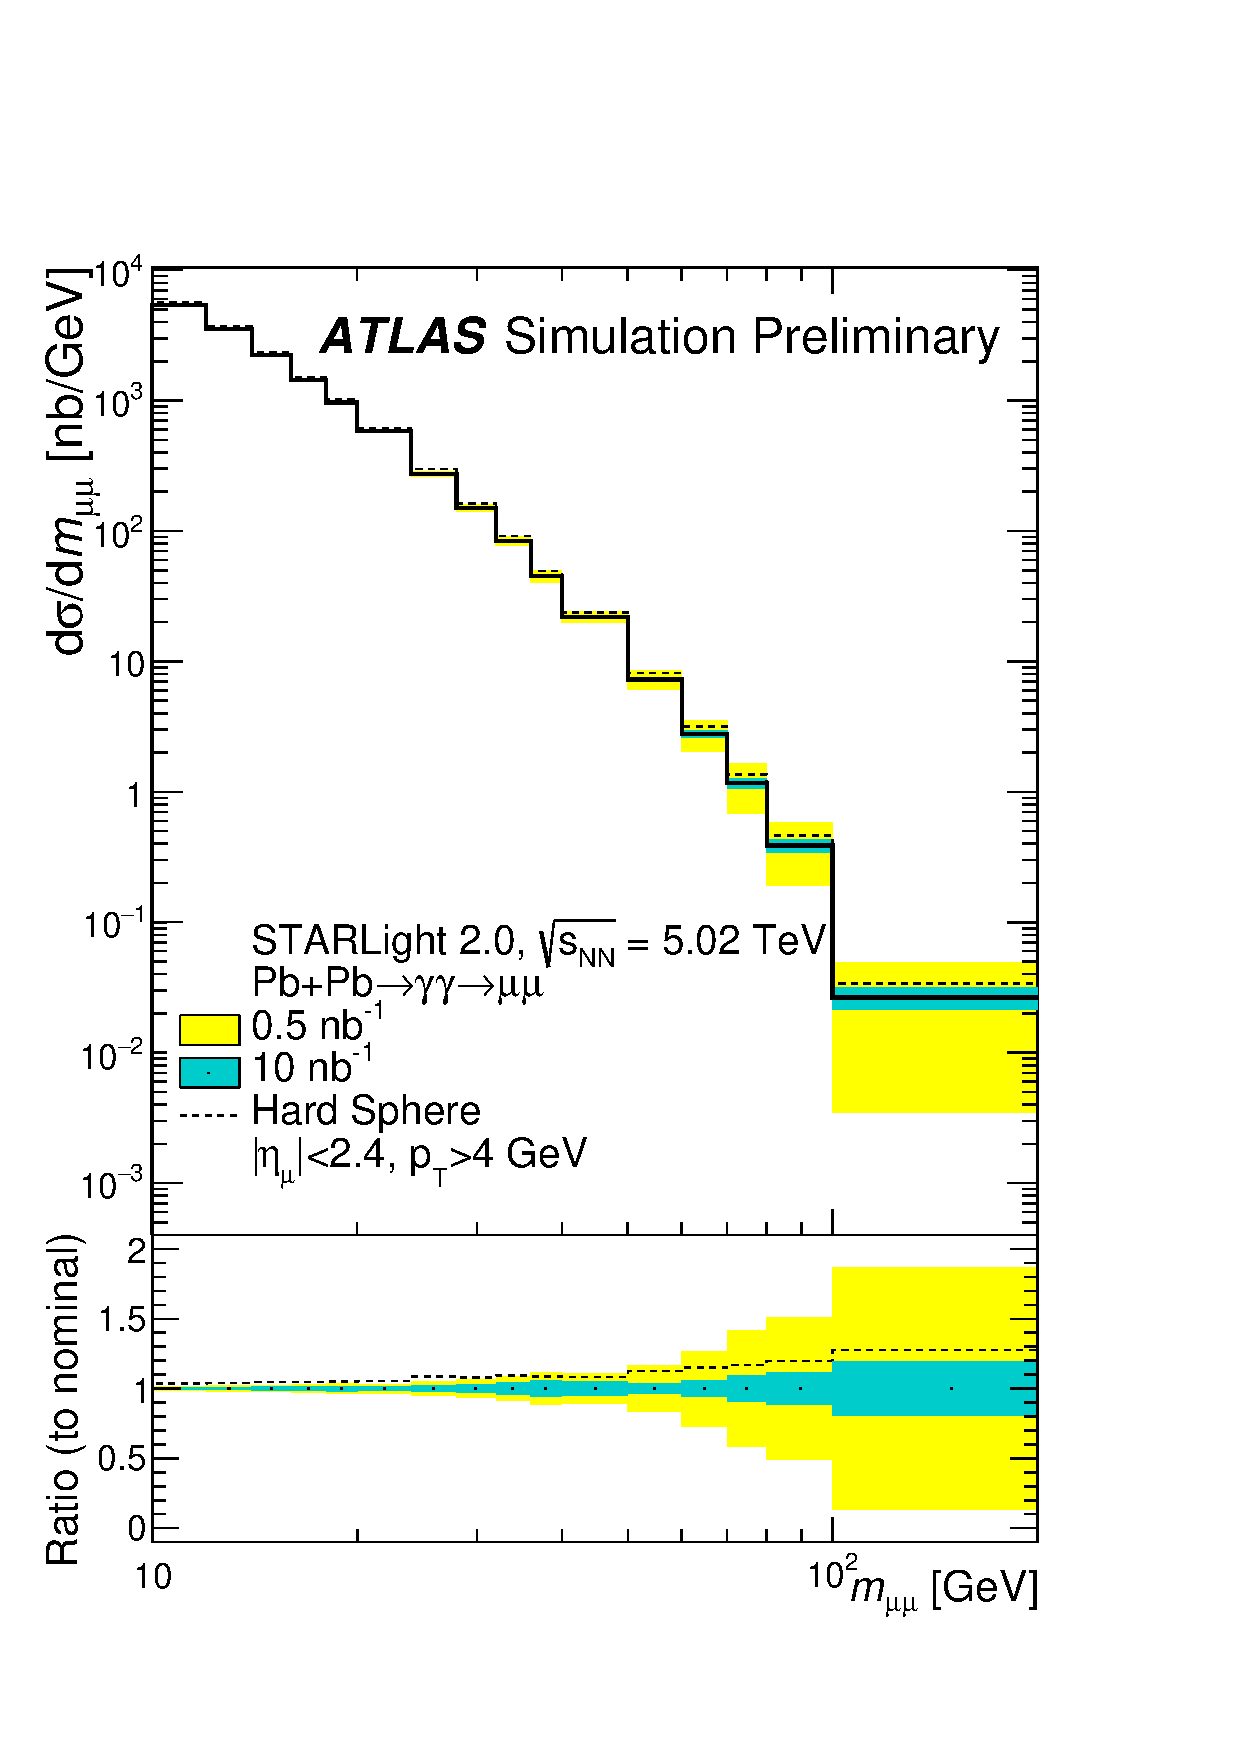
\includegraphics[width=0.50\linewidth]{\main/beyond/fig/fig_01.pdf}
\caption{
(Upper)~Differential cross section for exclusive production of the di-muon pairs as a function of the di-muon mass for
$10<m_{\mathrm{\mu\mu}}<200$~GeV extracted from STARLight. Two
scenarios are considered for the nuclear geometry: a realistic skin
depth of the nucleus~(solid line) or a hard sphere~(dashed
line). (Bottom)~Ratio to nominal as a function of the di-muon mass,
where "nominal'' stands for the realistic skin depth of the nucleus.
 Shaded bands represent expected statistical uncertainties associated with a number of signal events in each bin for integrated luminosity of $0.5~\mathrm{nb}^{-1}$~(yellow), and $10~\mathrm{nb}^{-1}$~(cyan).}
\label{fig:mumu}
\end{figure}
%-------------------------------------------------------------------

Exclusive production of di-muon pairs~($\mathrm{\gamma\gamma\rightarrow \mu^+\mu^-}$) in UPC can offer a precision measurement of photon fluxes associated with ion beams, and as such can be used to constrain predictions for the other processes covered in this section. The cross section at high pair mass is also sensitive to the nuclear geometry assumed in the calculations. Figure~\ref{fig:mumu} presents a differential cross section as a function of the invariant mass of the di-muon system in the range of 10-200~GeV with expected statistical uncertainties represented by two bands corresponding to integrated luminosities of $0.5~\mathrm{nb}^{-1}$ and
$10~\mathrm{nb}^{-1}$. Two scenarios are considered for the nuclear
geometry: a realistic skin depth of the nucleus or a hard sphere~\cite{Barrett:1977}.
For the $10~\mathrm{nb}^{-1}$ scenario, a significant reduction of the statistical uncertainty is expected. 
%In particular, in the highest $m_{\mathrm{\mu\mu}}$ bin which spans 100-200~GeV the uncertainty .  
This will help in reducing uncertainties from the modelling of the nuclear geometry.
The expected upgrades of the ATLAS Zero Degree Calorimeters~(ZDC) in the LHC Run 3 will also be important for isolating the contributions to the cross section stemming from dissociative processes.

Exclusive production of p$\mathrm{\bar{p}}$ pairs~($\mathrm{\gamma\gamma\rightarrow p\bar{p}}$) in heavy-ion collisions is considered as a process which can help verify the existing theoretical approaches. It has been demonstrated that the  $\mathrm{\gamma\gamma\rightarrow p\bar{p}}$ experimental data~\cite{Kuo:2005nr} from the Belle Collaboration can be successfully described by implementation of several components~\cite{Klusek-Gawenda:2017lgt}: the non-resonant proton exchange, $s$-channel tensor meson exchange and the hand-bag model~\cite{Diehl:2002yh}. Figure~\ref{fig:ppbar} shows the calculated distributions of invariant mass of the p$\mathrm{\bar{p}}$ system, $W_{\mathrm{\gamma\gamma}} = M_{\mathrm{p\bar{p}}}$~(left panel) and of the difference of rapidities for protons and anti-protons, $y_{\mathrm{diff}} = y_\mathrm{p} - y_{\mathrm{\bar{p}}}$~(right panel).
The ALICE Collaboration can measure p$\mathrm{\bar{p}}$ pairs in Pb--Pb collisions at mid-rapidity~($|y|$ < 0.9). 
The LHCb Collaboration could also provide a complementary measurement of p$\mathrm{\bar{p}}$ production in the forward region~(2 <$\eta$ < 4.5).
The upgraded charged particle tracking capabilities of ATLAS and CMS experiments for Run~4 will measure in $|y|<4.0$.
Corresponding kinematic requirements on transverse momenta and rapidity or pseudorapidity specific for each experiment are presented in the figure legend. The calculations are made for Pb--Pb collisions with $\sqrt{s_{\mathrm{NN}}}$ = 5.52~TeV.
The total cross section predicted for the ATLAS and CMS acceptances for $\pt>0.2$~GeV~($\pt>0.5$~GeV) is $\sigma$ = 793~$\mu$b~(248~$\mu$b), while LHCb and ALICE requirements lead to $\sigma$ = 125 and 105~$\mu$b, respectively.

%-------------------------------------------------------------------
\begin{figure}[!h]
        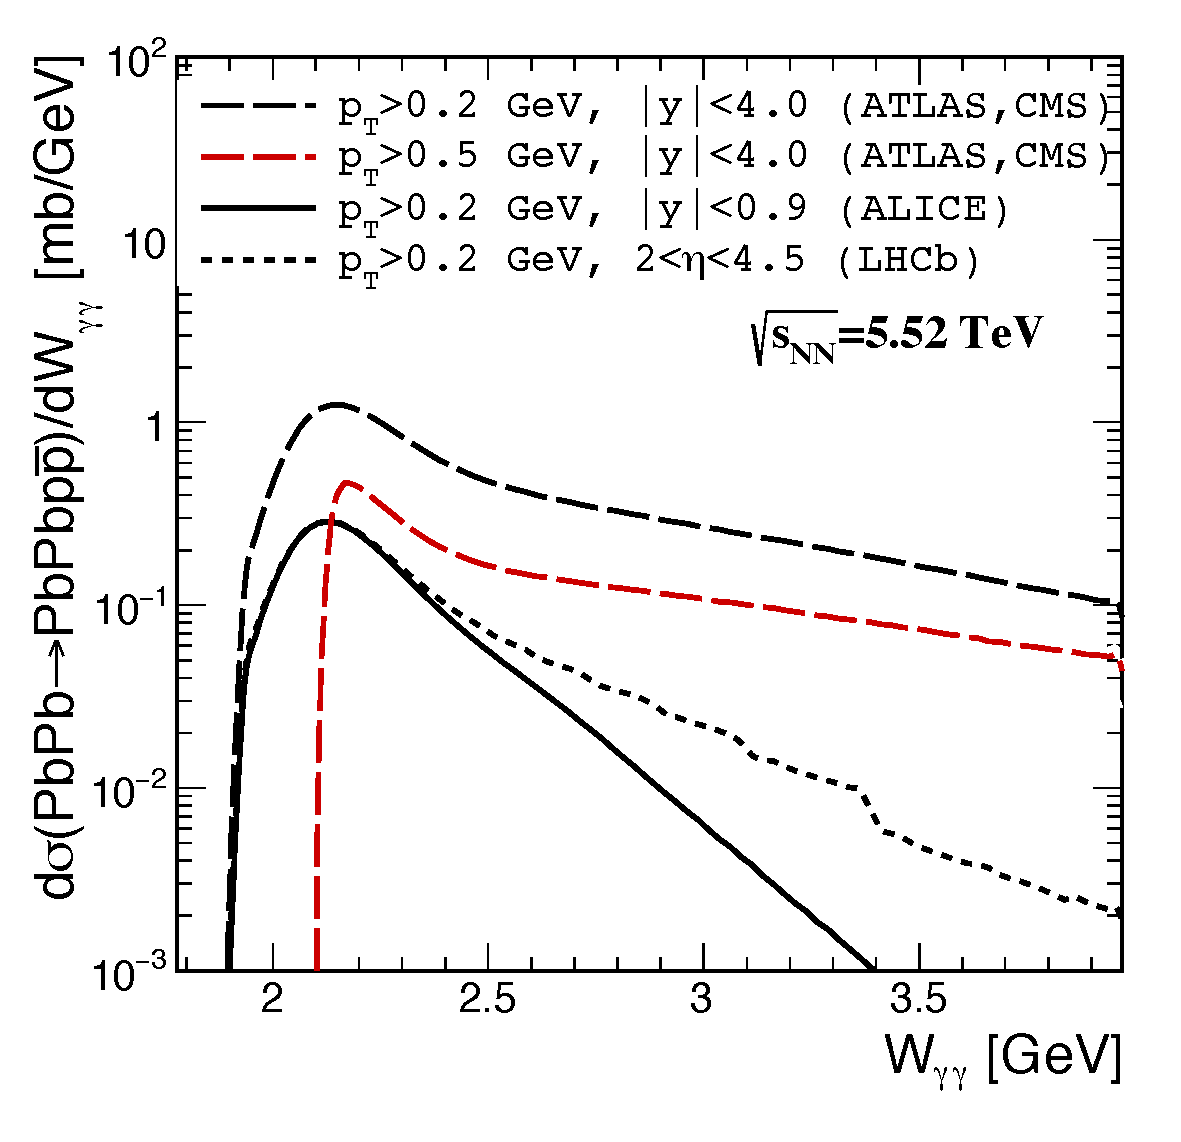
\includegraphics[scale=0.375]{\main/beyond/fig/dsig_dw_4exp_plus_y4_nucl_5520GeV.pdf}
        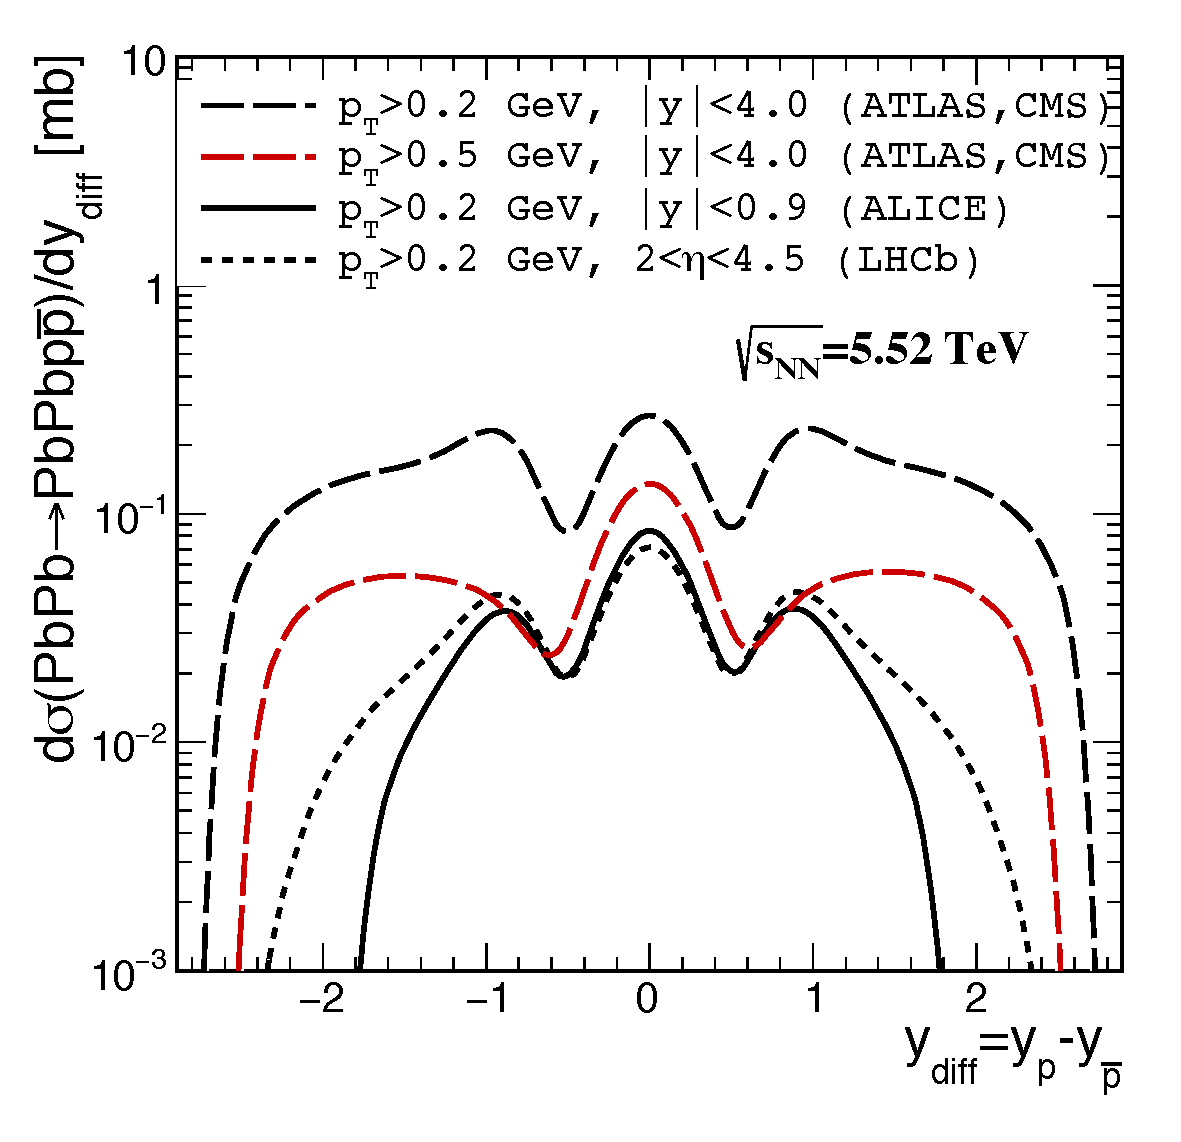
\includegraphics[scale=0.375]{\main/beyond/fig/dsig_dydiff_4exp_plus_y4_nucl_5520GeV.pdf}
        \caption{
                Differential cross sections as a function of $\mathrm{p\bar{p}}$
                invariant mass~(left) and rapidity
                distance between proton and anti-proton~(right)
                in Pb--Pb collisions at $\sqrt{s_{\mathrm{NN}}}$=5.52\,TeV
                for four experimental acceptance requirements. 
                For ATLAS and CMS experiments two requirements for proton $\pt>0.2$~GeV or $\pt>0.5$~GeV are considered.
        }
        \label{fig:ppbar}
\end{figure}
%-------------------------------------------------------------------


From the left panel of Figure~\ref{fig:ppbar} one can deduce that the dependence on invariant mass of the $\mathrm{p\bar{p}}$ pair is sensitive to the rapidity/pseudorapidity of the outgoing particle. The cut-off at the minimal value of $W_{\mathrm{\gamma\gamma}}$ is determined by the minimum $\pt$ requirement.
The $y_{\mathrm{diff}}$ distribution shown in the right panel of Figure~\ref{fig:ppbar} is of particular interest. 
The broad maximum at $y_{\mathrm{diff}}=0$ corresponds to the region with $|\cos \theta|$ < 0.6, where $\theta$ denotes the angle of the outgoing nucleon relative to the beam direction in the centre-of-mass frame.  
An observation of peaks at $y_{\mathrm{diff}} = \pm 1$ could be a good test to constraint the theoretical models which predict the elementary cross section. The proposed model has a few parameters~(i.e. vertex form factors for the proton exchange, tensor meson s-channel exchanges and a form factor in the hand-bag contribution) which could be constrained with the help of the $y_{\mathrm{diff}}$ distributions.
The fiducial acceptance requirements imposed on $\pt$ do not distort the maxima.
If the structures in the $y_{\mathrm{diff}}$ distributions indeed exist, the study of $\mathrm{p\bar{p}}$ production in UPC can provide an important complimentary information  to the existing $\mathrm{\gamma\gamma\rightarrow J/\psi \rightarrow e^+e^-}$ production data~\cite{Kryshen:2017jfz,Abbas:2013oua}.


Evidence of the rare process of LbyL scattering has been established by the ATLAS and CMS Collaborations using Pb--Pb data obtained in 2015~\cite{Aaboud:2017bwk,Sirunyan:2018fhl} with an integrated luminosity of about $0.4\;\mathrm{nb}^{-1}$. That process can be studied with higher precision using heavy-ion data collected at the HL-LHC. The left panel of Figure~\ref{fig:lbyl} presents a differential cross section as a function of the di-photon rapidity for LbyL scattering for photons with $|\eta^{\mathrm{\gamma}}|<4$ with two photon $\pt^{\mathrm{\gamma}}$ thresholds: 2.0 and 2.5~GeV. The LbyL scattering occurs in the central region: 91\% of the integrated cross section resides within $|\eta^{\mathrm{\gamma}}|<2.37$. A strong dependence on the $\pt^{\mathrm{\gamma}}$ requirement is observed. The cross section increases by a factor of two when the single photon $\pt^{\mathrm{\gamma}}$ threshold is lowered by half a GeV from 2.5 to 2.0~GeV. The corresponding integrated cross sections in the fiducial region are 112~nb for $\pt^{\mathrm{\gamma}}>2.5$~GeV and 221~nb for $\pt^{\mathrm{\gamma}}>2.0$~GeV. 

The right panel of Figure~\ref{fig:lbyl} shows a detector-level acoplanarity~(=$1-|\varphi^{\mathrm{\gamma}}_1-\varphi^{\mathrm{\gamma}}_2|/\pi$) distribution for the di-photon system from LbyL signal and two background processes originating from exclusive production of di-electron pairs~($\mathrm{\gamma\gamma\rightarrow\,e^+e^-}$) and di-photons produced in central exclusive production~($\mathrm{gg\rightarrow \gamma\gamma}$). The distributions depict simulated events which passed a full simulation of the ATLAS detector with the extended acceptance in pseudorapidity. About 640 LbyL events pass the selection requirements for acoplanarity below 0.01 and $\pt^{\mathrm{\gamma}}>2.5$~GeV in 5.02~TeV Pb--Pb~collisions with an integrated luminosity of 10\,nb$^{-1}$, in comparison to about 13 events observed in the 2015 data set with the $\pt^{\mathrm{\gamma}}>3.0$~GeV requirement. 
The signal events are peaked at acoplanarities close to zero, while the background processes are distributed either uniformly (di-photons from central exclusive production) or even grow with acoplanarity~($\mathrm{e^+e^-}$ pairs from exclusive di-electron production). The latter originates from $\mathrm{e^+e^-}$ pairs which trajectories have been bent in the magnetic field before emitting hard-bremsstrahlung photons.
A limitation of the current analysis is lack of simulation of the trigger response. Based on experience from the analyses of 2015 Pb--Pb data, triggering on photons with $\pt^{\mathrm{\gamma}}<3.0$~GeV is challenging, and therefore a dedicated trigger strategy needs to be developed for LbyL event candidates exploiting new features of the upgraded trigger system~\cite{Aad:2013tqj,Tapper:1556311}.

%-------------------------------------------------------------------
\begin{figure}[!hbt]
\centering
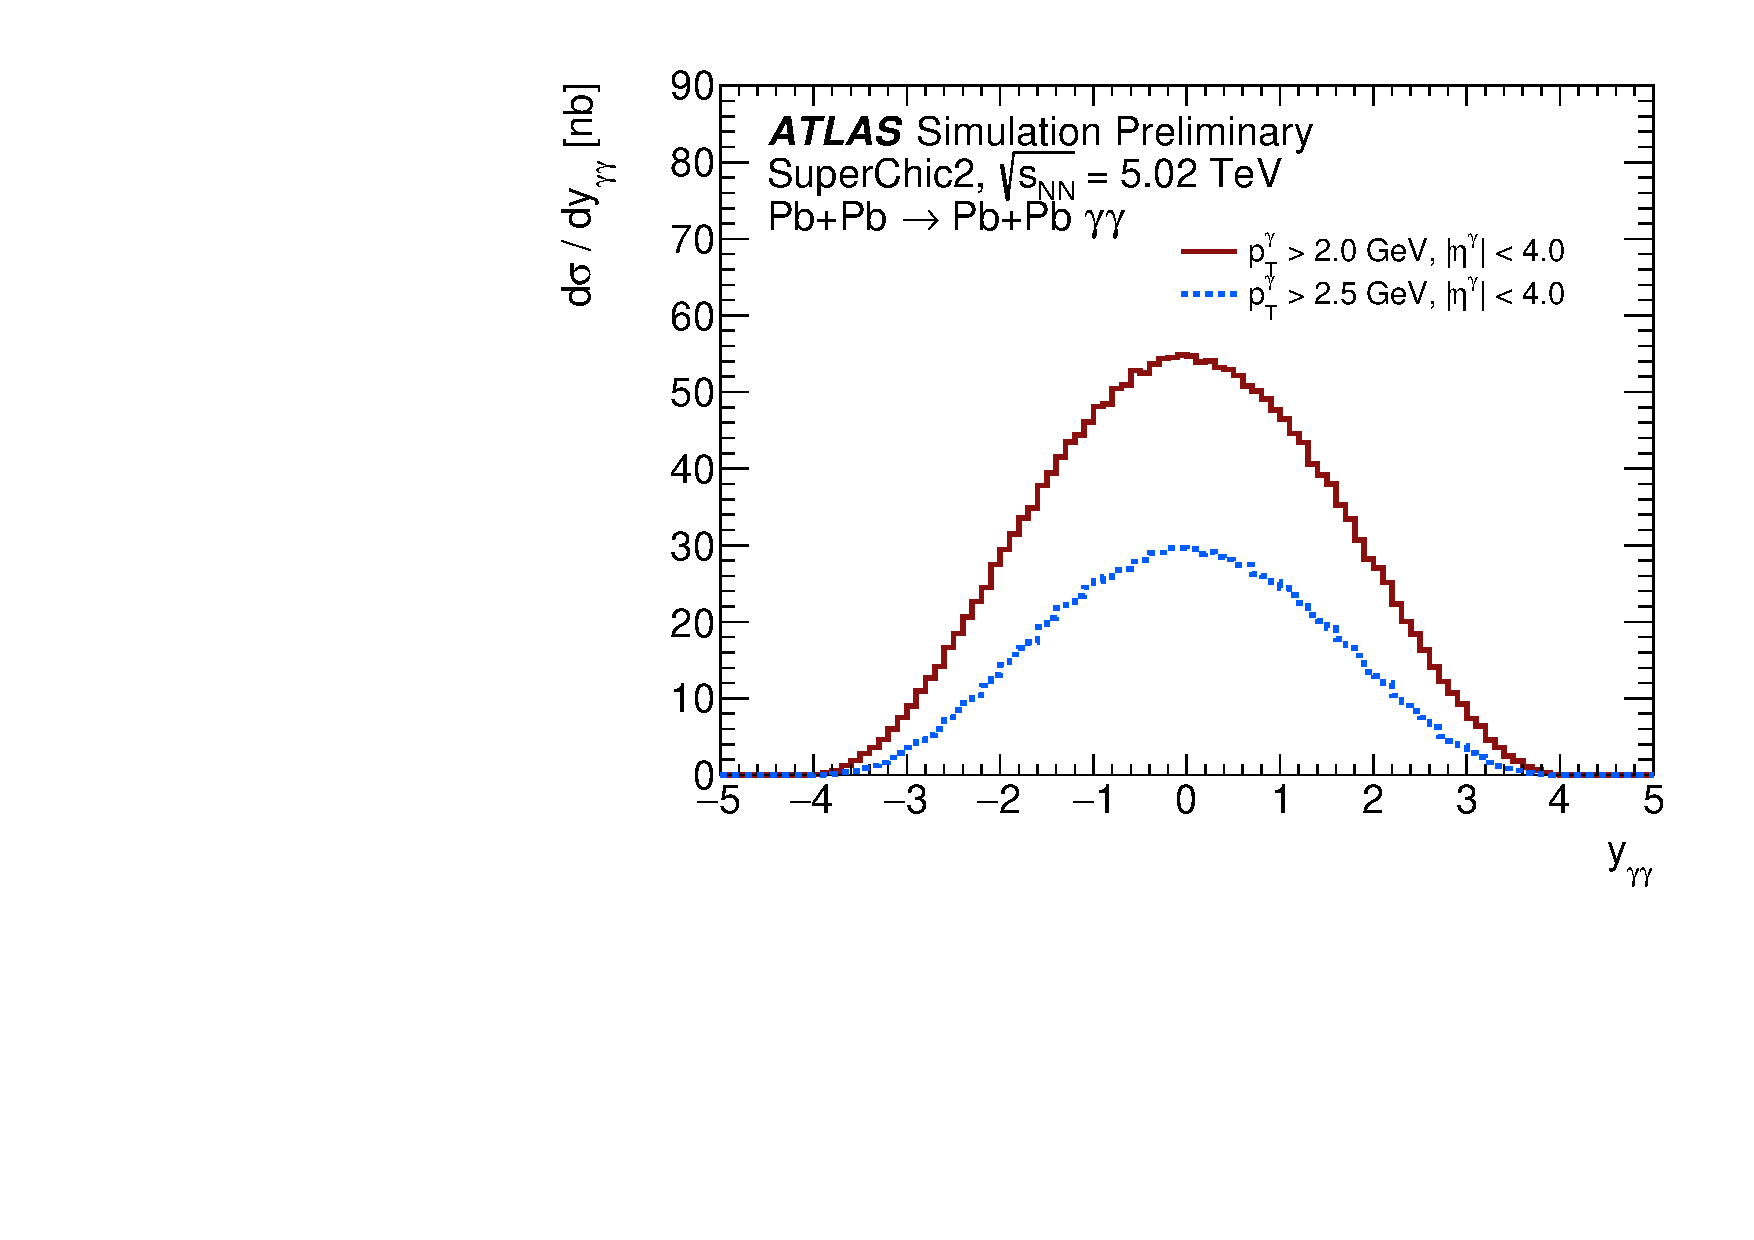
\includegraphics[width=0.49\linewidth]{\main/beyond/fig/fig_02.pdf}
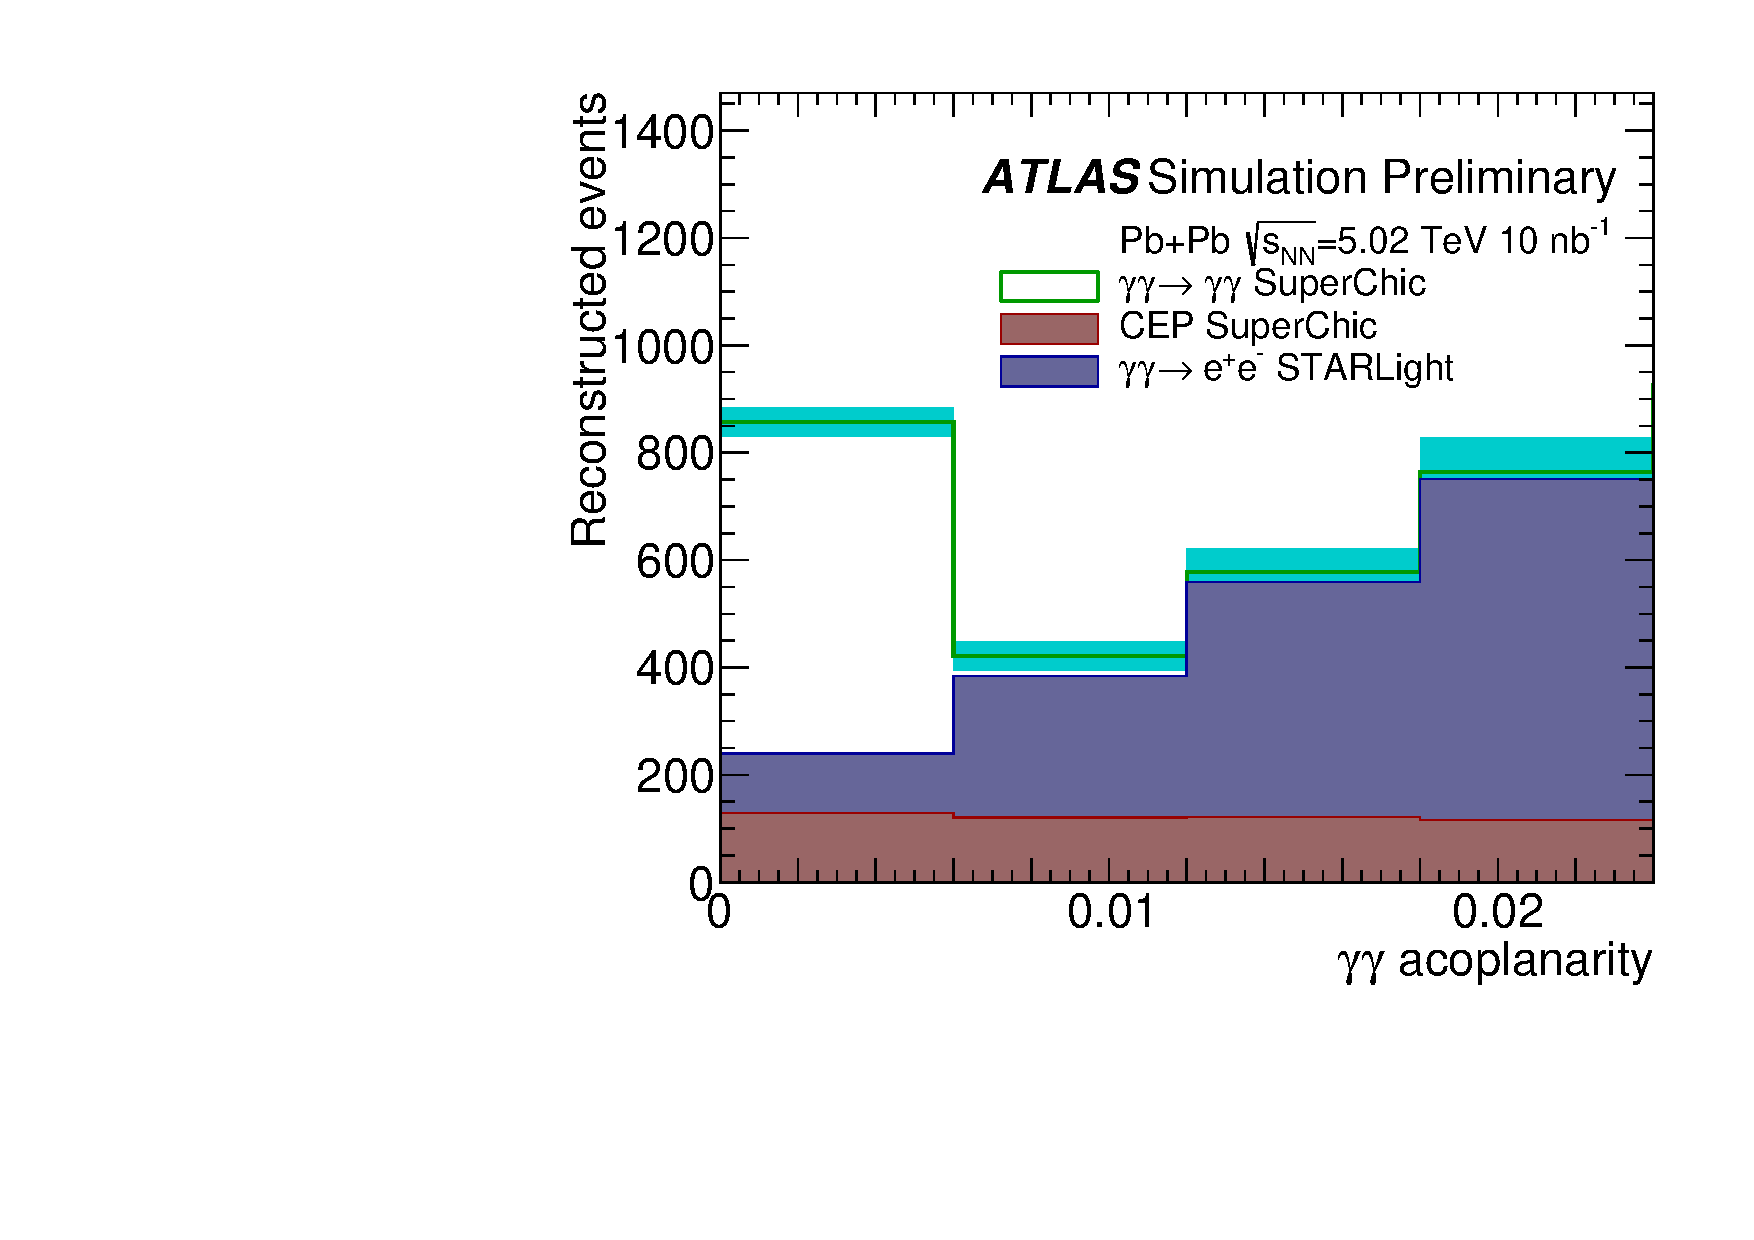
\includegraphics[width=0.425\linewidth]{\main/beyond/fig/fig_03a.pdf}
\caption{
(Left)~Predicted differential cross section as a function of the di-photon rapidity for LbyL scattering for photons with
$\pt^{\mathrm{\gamma}}>2.5$~GeV~(dashed) or $\pt^{\mathrm{\gamma}}>2.0$~GeV~(solid), and
$|\eta^{\mathrm{\gamma}}|<4$ extracted from SuperChic~\cite{Harland-Lang:2018iur}.
(Right) Detector-level acoplanarity distribution of the di-photon system for photons from the LbyL signal and background processes in
  5.02~TeV Pb--Pb collisions with an integrated luminosity of
  $10~\mathrm{nb}^{-1}$. The shaded band in cyan represents expected statistical uncertainties.
}
\label{fig:lbyl}
\end{figure}
%-------------------------------------------------------------------

The LbyL process can also be studied at lower di-photon masses. The differential cross sections as a function of the di-photon mass can be evaluated taking into account acceptance of the ALICE experiment, i.e. pseudorapidity limited to $|\eta^{\mathrm{\gamma}}|<0.9$ or in the forward region defined by $2<\eta^{\mathrm{\gamma}}<4.5$ in the LHCb experiment, and relatively low energies of outgoing photons~\cite{Abelev:2014ypa}. At lower energies~($W_{\mathrm{\gamma\gamma}} <$ 4~GeV) meson resonances~\cite{Klusek-Gawenda:2018ijg} may play an important role in addition to the Standard Model box diagrams~\cite{dEnterria:2013zqi,Klusek-Gawenda:2016euz} or double photon fluctuations into light vector mesons~\cite{Klusek-Gawenda:2016euz} or two-gluon exchanges~\cite{Klusek-Gawenda:2016nuo}.
%-------------------------------------------------------------------
\begin{figure}[!h]
        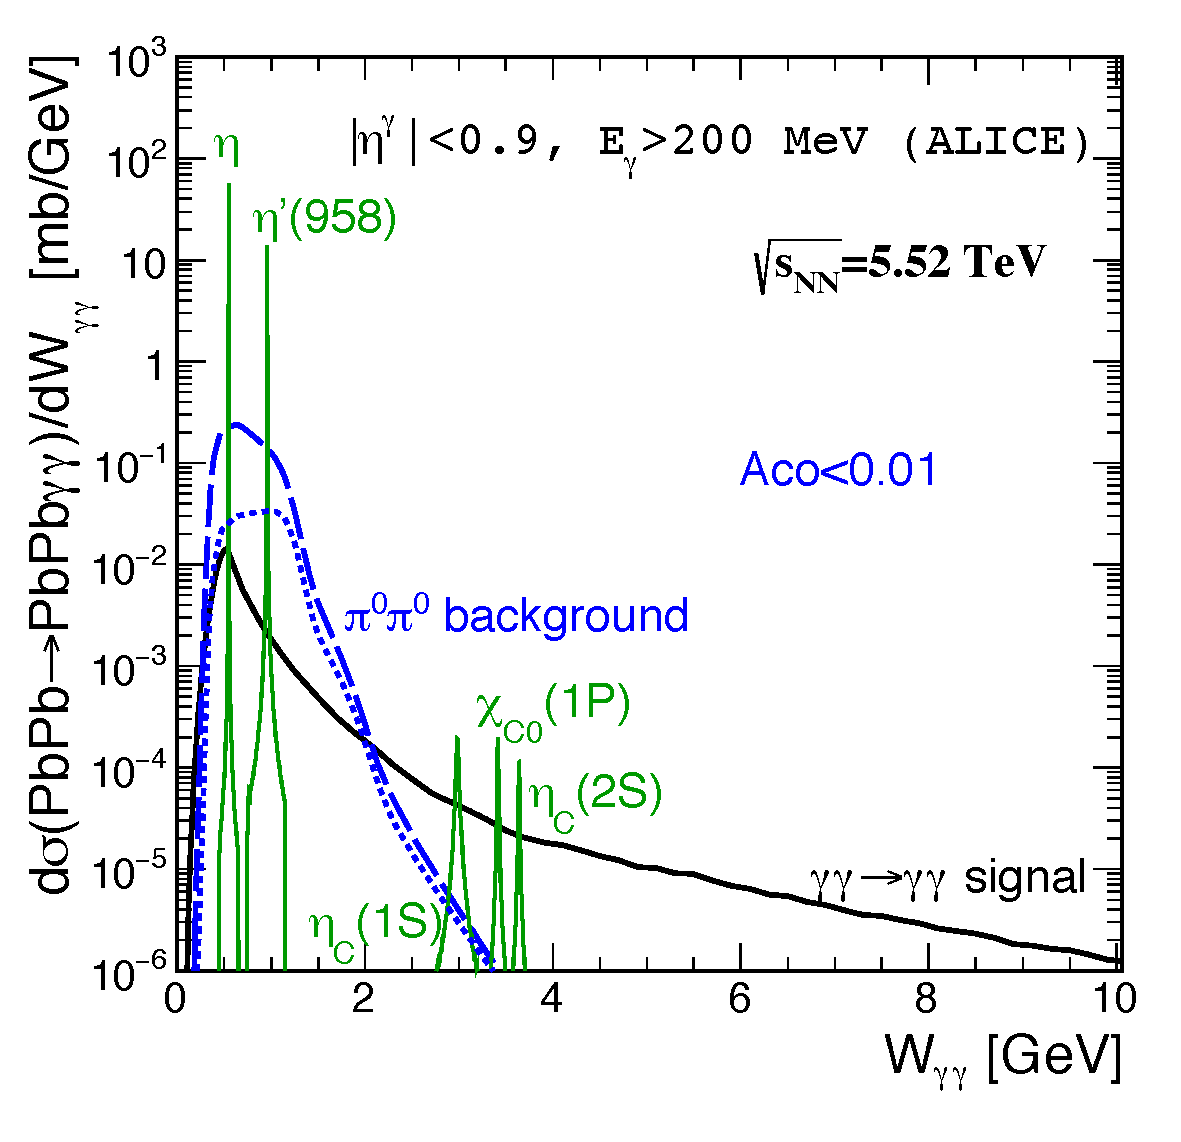
\includegraphics[scale=0.375]{\main/beyond/fig/dsig_dW_LbL_Pb_ALICE_aco001.pdf}%
        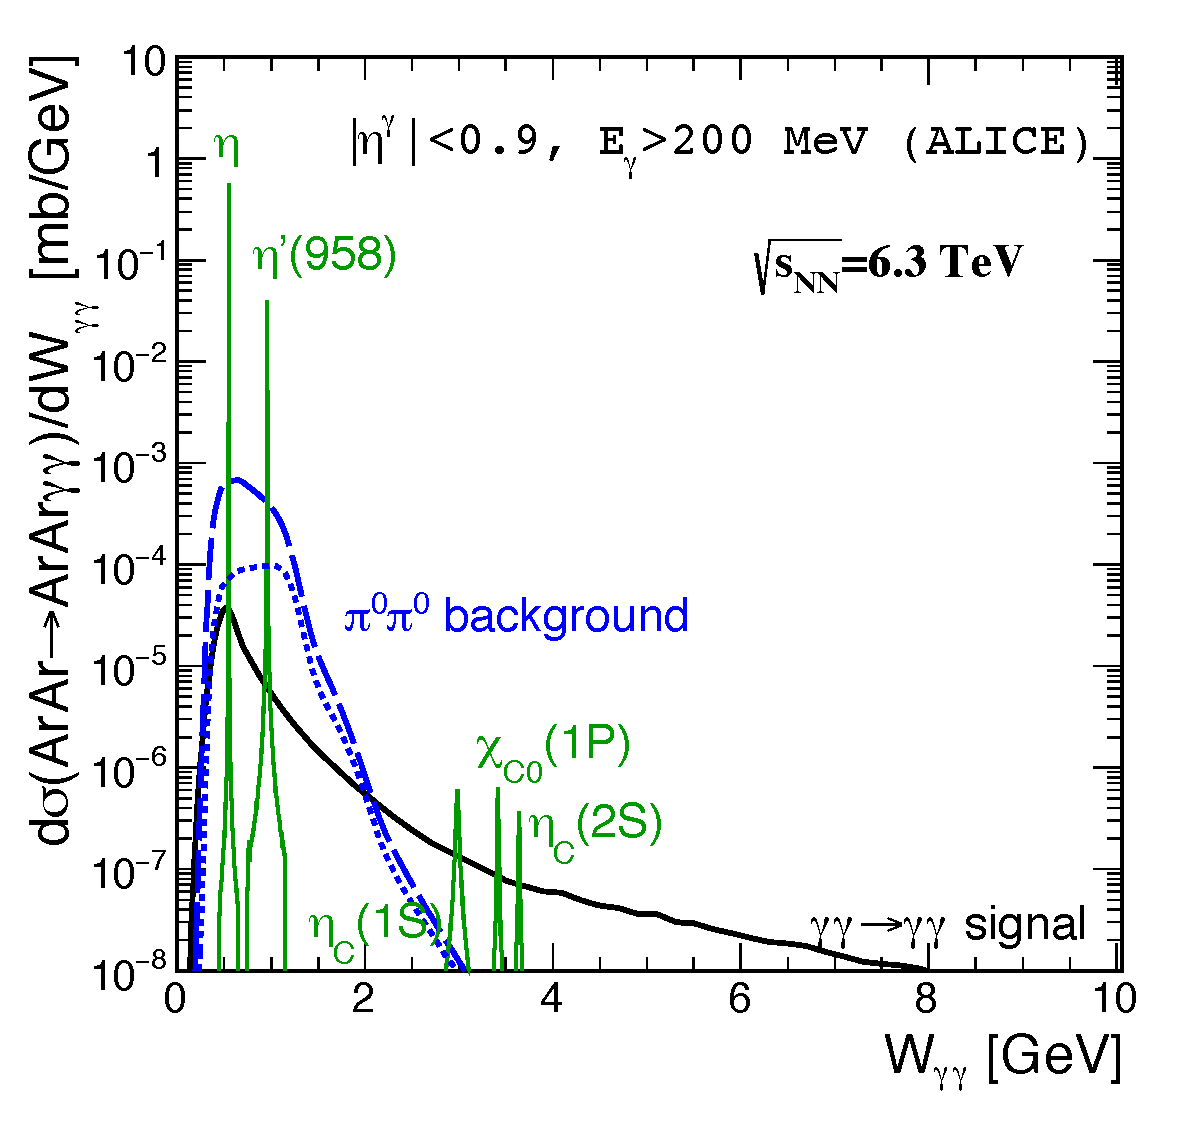
\includegraphics[scale=0.375]{\main/beyond/fig/dsig_dW_LbL_Ar_ALICE_aco001.pdf}\\
        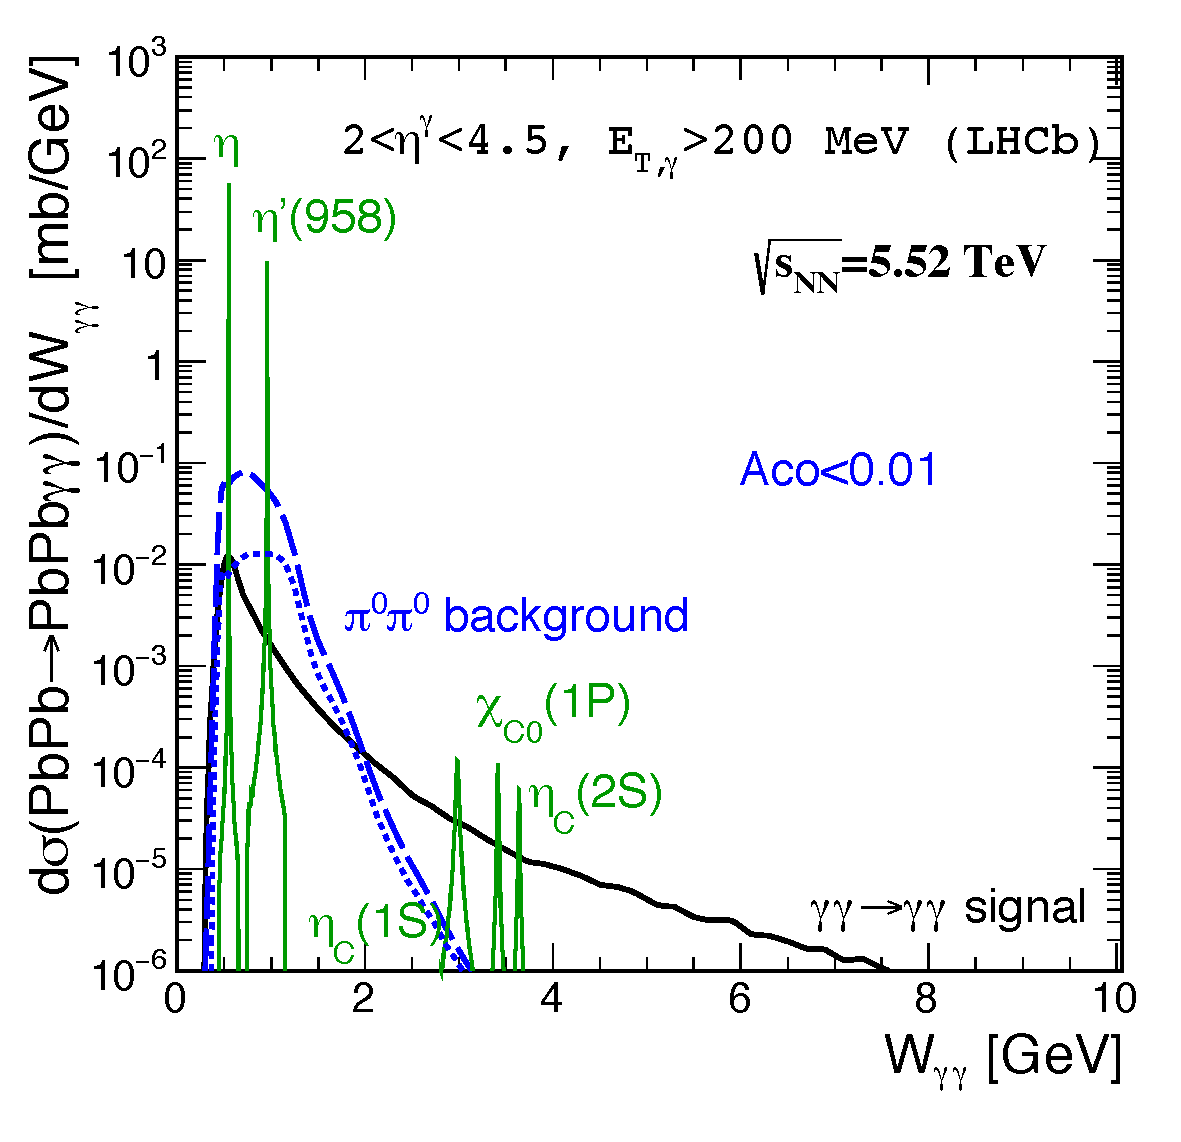
\includegraphics[scale=0.375]{\main/beyond/fig/dsig_dW_LbL_Pb_LHCb_aco001.pdf}%
        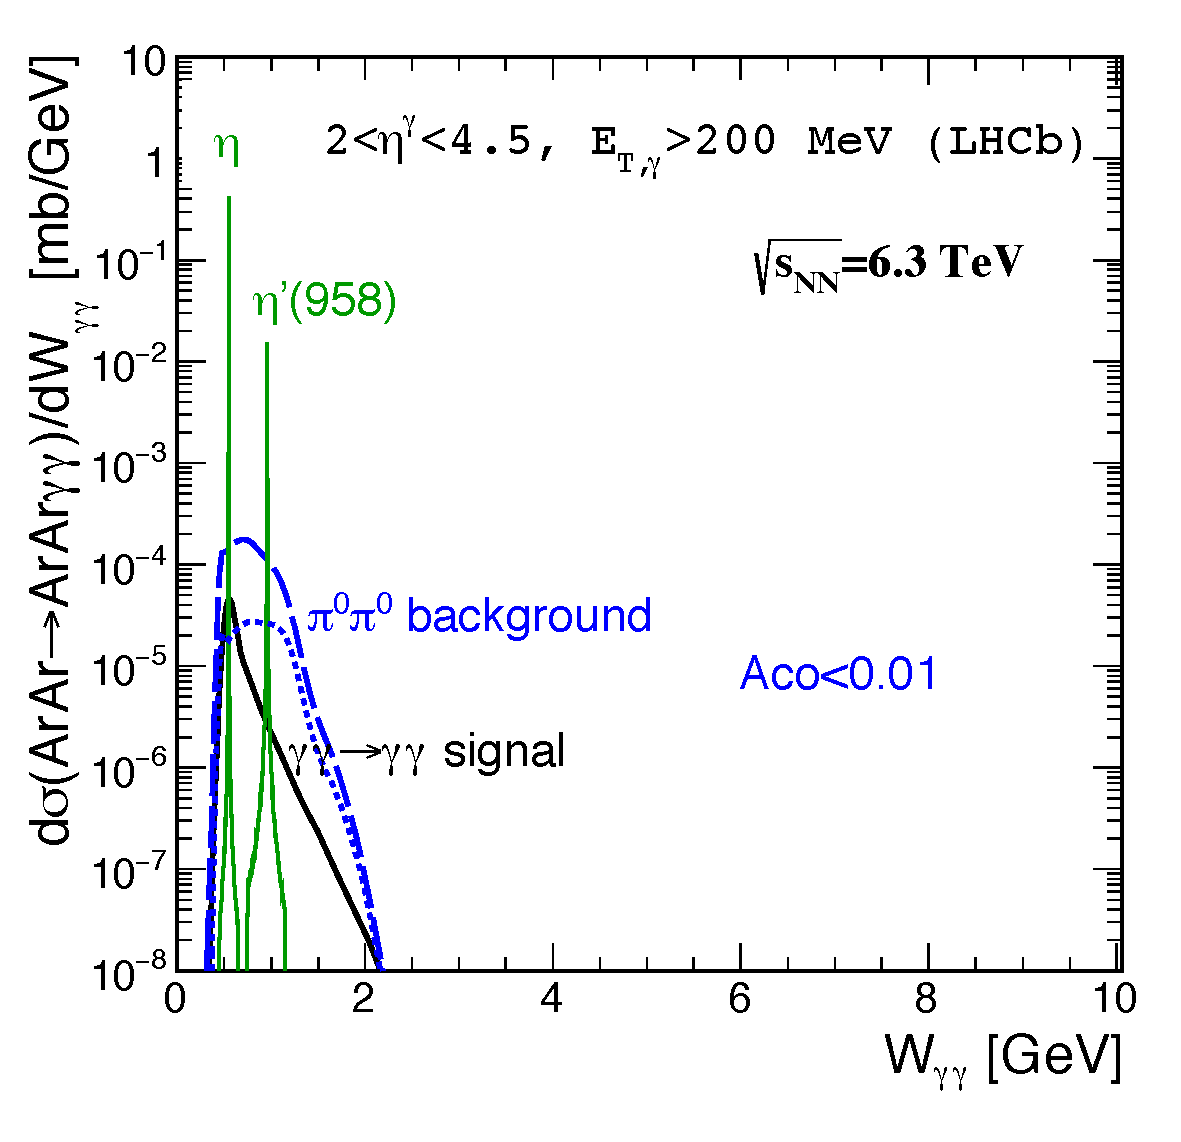
\includegraphics[scale=0.375]{\main/beyond/fig/dsig_dW_LbL_Ar_LHCb_aco001.pdf}
        \caption{
                Di-photon invariant mass distributions for Pb--Pb collisions at $\sqrt{s_{\mathrm{NN}}}$=5.52\,TeV~(left) and Ar--Ar collisions at $\sqrt{s_{\mathrm{NN}}}$=6.3\,TeV~(right) for ALICE at mid-rapidity~(top) and LHCb at forward pseudorapidity~(bottom). The $\mathrm{\pi^0\pi^0}$ background is shown with the acoplanarity requirement of 0.01~(dotted line) and also without it~(dashed line).}
        \label{fig:lbyl_alice}
\end{figure}
%-------------------------------------------------------------------
Figure~\ref{fig:lbyl_alice} shows predictions for LbyL and background processes in the ALICE and LHCb experiments with photon acceptance in $|\eta^{\mathrm{\gamma}}|<0.9$ and $E_{\mathrm{\gamma}}$ > 200~MeV~(top panel) or $2<\eta^{\mathrm{\gamma}}<4.5$ and $E_{\mathrm{T,\gamma}}$ > 200~MeV~(bottom panel), respectively, for two systems: Pb--Pb collisions at 5.52~TeV~(left panel) and Ar--Ar collisions at 6.3~TeV~(right panel). Presented results include the effect of the experimental energy resolution~\cite{Acharya:2018yhg,Govorkova:2015vqa}. The black-solid lines depict the LO QED fermionic box mechanism with leptons and quarks. Presented results for the $\mathrm{\gamma\gamma\to\gamma\gamma}$ process are in agreement with calculations from Refs.~\cite{Jikia:1993tc,Bern:2001dg,Bardin:2009gq}. The green-solid lines show results for the $s$-channel $\mathrm{\gamma\gamma}\to$pseudoscalar/scalar/tensor resonances that contribute to the LbyL process.
In the present analysis, $\eta$, $\eta'(958)$, $\eta_c(1S)$, $\eta_c(2S)$, $\chi_{c0}(1P)$ mesons are considered.
Their masses, total widths and branching ratios are taken from the PDG~\cite{Patrignani:2016xqp}.
The dominant background from the $\mathrm{\gamma\gamma\to\pi^0\pi^0}$
process is depicted by the blue lines. It becomes non-negligible only when one photon from each $\mathrm{\pi^0\to\gamma\gamma}$ decay is reconstructed in the detector. Two scenarios with and without the acoplanarity requirement of 0.01 are considered. The acoplanarity requirement reduces this background contribution by a factor of 5 in the full $W_{\mathrm{\gamma\gamma}}$ region.
The experimental data for the $\mathrm{\gamma\gamma\to\pi\pi}$ elementary cross section were very well described in Ref.~\cite{Klusek-Gawenda:2013rtu}.
There simultaneously the total cross section and angular distributions for both charged and neutral pions are shown.
Following Ref.~\cite{Klusek-Gawenda:2013rtu}, here nine resonances,
$\mathrm{\gamma\gamma\to\rho^\pm\to\pi^0\pi^0}$ continuum, Brodsky-Lepage and hand-bag mechanism are included. Figure~\ref{fig:lbyl_alice} shows that pionic background dominates at low invariant di-photon mass~(below 2~GeV).
In the same energy region, one can observe a very clear dominance of
$\mathrm{\eta}$, $\mathrm{\eta'(958)}$ mesons over other processes.
The inclusion of energy resolution introduces mainly smearing of the contribution from
$\mathrm{\gamma\gamma\to\eta,\eta'\to\gamma\gamma}$ resonance scattering.
This contribution is supposed to be measured with good precision.
%However, the resonance signal is modified including experimental energy resolution and a peak is about one order of magnitude smaller than without experimental resolution but the total cross section is of course still the same.
These results suggest that both ALICE and LHCb Collaborations could measure LbyL scattering for $W_{\mathrm{\gamma\gamma}}>$ 2~GeV in Pb--Pb collisions. The cross sections are about two orders of magnitude lower in the Ar--Ar system due to smaller electric charge associated with argon beams. Assuming integrated luminosities of $3.0-8.8$~$\mathrm{pb^{-1}}$ in a dedicated Ar--Ar run, the LbyL production cross section leads to 1460-4280 signal events for ALICE and 11-34 events for LHCb in a range of $W_{\mathrm{\gamma\gamma}}>2$~GeV. A background contribution from $\mathrm{\gamma\gamma\to\pi^0\pi^0}$ is at the level of 20\% for ALICE and 134\% for LHCb in this region.


Axions and axion-like particles~(ALP) are fundamental components of extensions of the Standard Model, occurring in most solutions of the strong CP problem~\cite{Peccei:1977hh,PhysRevLett.38.1440}. Recently an increasing interest has been paid to ALP masses
above 1~GeV~\cite{Bauer:2017ris,Mimasu:2014nea,Jaeckel:2015jla,Knapen:2016moh,Brivio:2017ije}. In particular the Higgs discovery has set spin zero particles in the spotlight of searches for new physics, with scalar and pseudo-scalar particles (elementary or not) as heralds of new phenomena. An interesting feature is that ALP (generically labelled as $\mathrm{a}$ in the following) in this mass range would induce an anomalous contribution to the LbyL, via the reaction:
$\mathrm{\gamma \gamma \rightarrow a \rightarrow \gamma \gamma}$,
under the condition that the magnitudes of the EM fields associated
with the incident photon are large enough, typically $|\vec{E}| >10^{18}$~V/m.
This has triggered  the study presented in Ref.~\cite{Knapen:2016moh},
and then in Ref.~\cite{Knapen:2017ebd} using the recent observation of LbyL scattering published by the ATLAS experiment in Pb--Pb collisions~\cite{Aaboud:2017bwk}, where the electric field produced by the ultra-relativistic Pb is of the order of $10^{25}$~V/m (thus satisfying the above condition).

The potential of ALP searches in UPC Pb--Pb collisions is studied using detector-level quantities after the LbyL selection requirements are imposed. The overall selection efficiency (times acceptance) relative to generated events increases from about $40$\% to $65$\% for ALP masses ranging from $7$~GeV to $80$~GeV. Also, the mass resolution varies from $0.5$~GeV at low masses (below $15$~GeV) up to $1$~GeV for larger masses. In the left panel of Figure~\ref{fig:alp} the expected mass distributions for three ALP signal mass values, and the main background from LbyL normalised to integrated luminosity of 10~$\mathrm{nb}^{-1}$ are shown. In this study, other sources of backgrounds are neglected, since they have been found to be small in the LbyL measurement~\cite{Aaboud:2017bwk}. The invariant mass distribution is used as the discriminating variable, with bin widths comparable to the expected resolution of a narrow resonant signal.
Upper limits are set on the product of the production cross section of
new resonances and their decay branching ratio into $\mathrm{\gamma\gamma}$. Exclusion intervals are derived using the CLs method~\cite{Read:2002hq} in the asymptotic approximation. The limit set on the signal strength $\mu$ is then translated into a limit on the signal cross section times branching ratio as presented in the right panel of Figure~\ref{fig:alp}.
%-------------------------------------------------------------------
\begin{figure}[!htbp]
\centering
  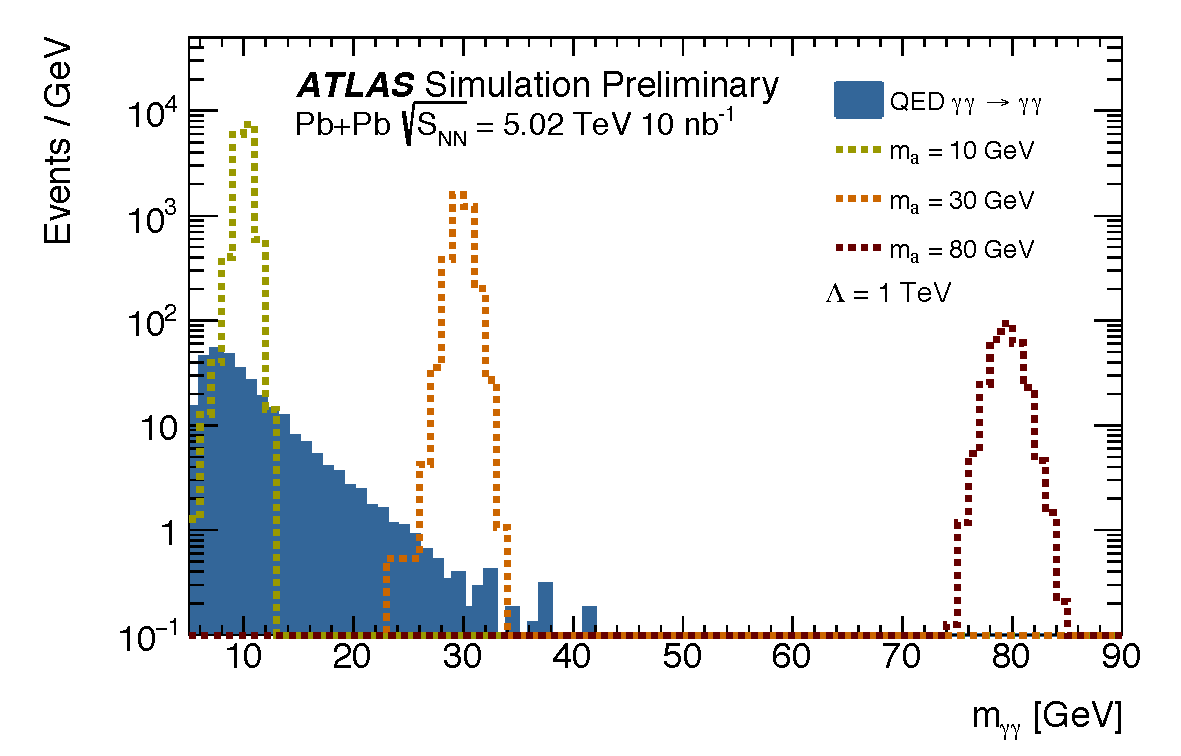
\includegraphics[scale=0.45]{\main/beyond/fig/fig_04.pdf}
  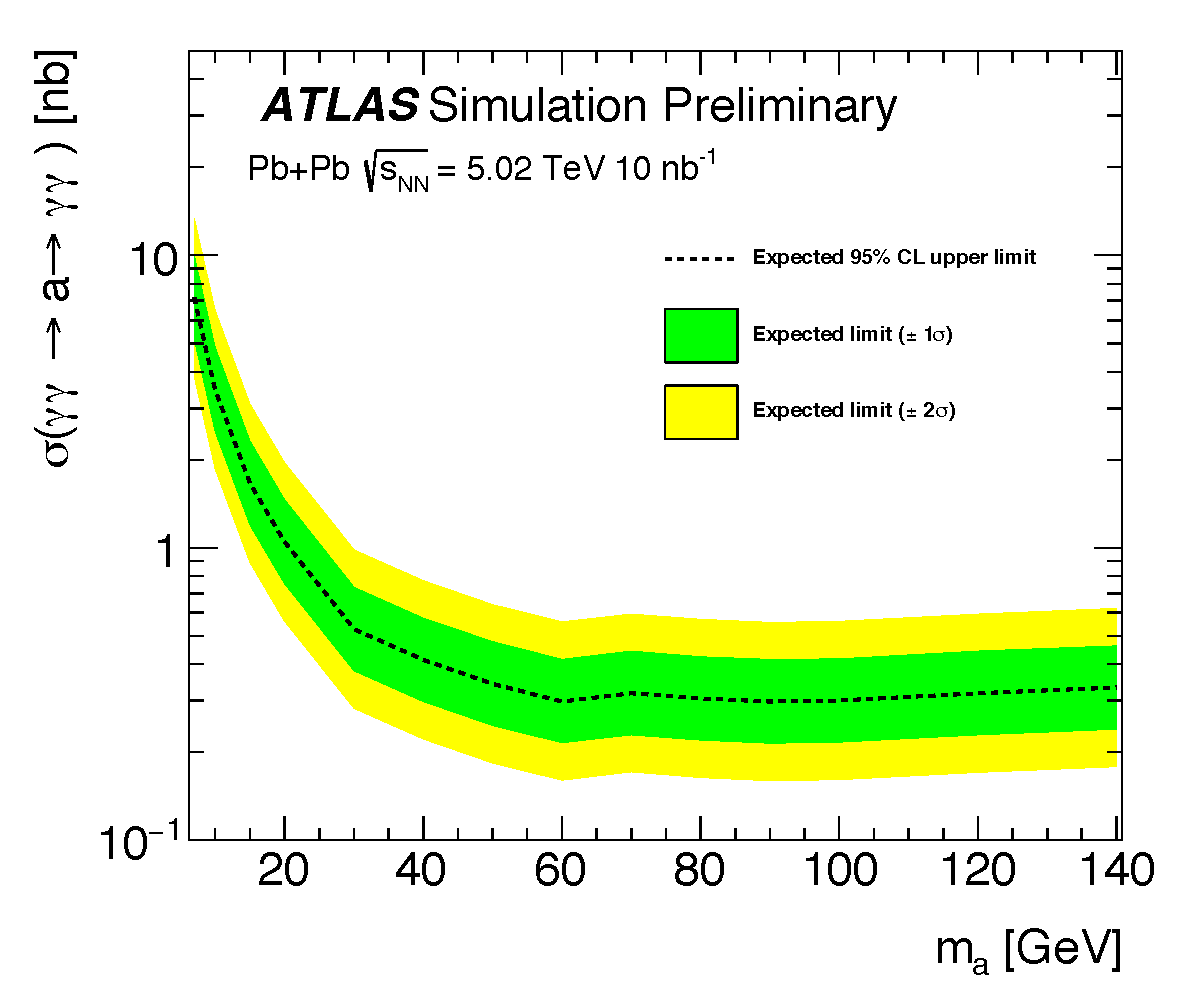
\includegraphics[scale=0.34]{\main/beyond/fig/fig_05a.pdf}
  \caption{(Left)~Mass distribution for the ALP signal
  shown for three values of the ALP mass: $m_\mathrm{a}=10, 30$ and
  $80$~GeV~(in red). Also shown (in blue) the LbyL background~(see
  text). All ALP mass points are generated with $\Lambda = 1$~TeV which follows a convention defined in Ref.~\cite{Knapen:2016moh}.
  (Right)~Expected $95$\% CLs upper limits on $\sigma_{\mathrm{a\rightarrow \gamma \gamma}}$.}
  \label{fig:alp}
\end{figure}
%-------------------------------------------------------------------

In Figure~\ref{fig:alp-lambda-limits-cms} exclusion limits on the coupling as a function of $m_\mathrm{a}$ are presented along with the existing results from the compilation discussed in Ref.~\cite{Baldenegro:2018hng}. The ATLAS 20~nb$^{-1}$ limit is derived using the analysis for Pb--Pb collisions at 5.52~TeV. These results demonstrate that heavy-ion collisions have unique sensitivity to ALP searches in the range of ALP masses between $7$~GeV and $140$~GeV, where the previous analysis~\cite{Knapen:2016moh} is also shown~(labelled as ATLAS 2016 in the figure).

%-------------------------------------------------------------------
\begin{figure}[!htbp]
\centering
  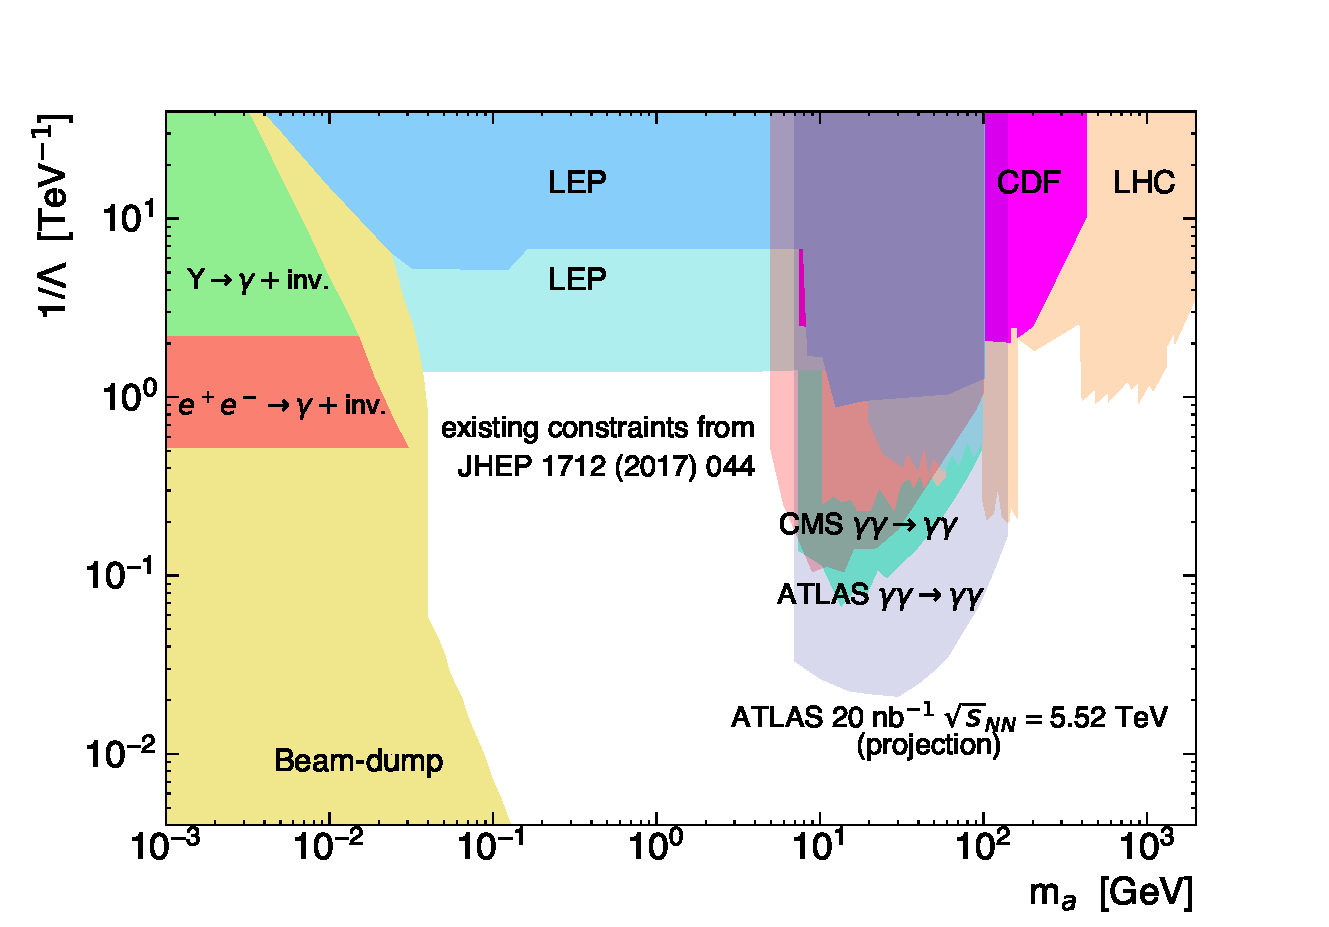
\includegraphics[scale=0.6]{\main/beyond/fig/Figure_atlas_cms_v2.pdf}
  \caption{Compilation of exclusion limits obtained by different experiments (see text). The ATLAS $\mathrm{\gamma\gamma\rightarrow\gamma\gamma}$ represents the exclusion limit derived from the recent LbyL cross section measured in Pb–-Pb collisions by ATLAS, while the CMS $\mathrm{\gamma\gamma\rightarrow\gamma\gamma}$ limit comes from the analysis done in Ref.~\cite{Sirunyan:2018fhl}. In light grey, the ATLAS 20 nb −1 limit for $\sqrt{s_{\mathrm{NN}}}=5.52$ = 5.52 TeV is presented. A more complete version of the existing constraints on ALPs masses versus coupling, including the constraints in the sub meV range from astrophysical observations and from dedicated experiments such as CAST can be found in Ref.~\cite{Bauer:2017ris}.}
  \label{fig:alp-lambda-limits-cms}
\end{figure}
%-------------------------------------------------------------------

%In Figure~\ref{fig:alp-lambda-limits} two exclusion limits on the coupling as a function of $m_\mathrm{a}$ are presented along with the existing results from the compilation discussed in Ref.~\cite{Baldenegro:2018hng}. The LHC 10~nb$^{-1}$ limit is derived using the analysis for Pb--Pb collisions at 5.02~TeV. The LHC 20~nb$^{-1}$ limit is established using a combined analysis of the ATLAS and CMS data assuming similar acceptance and photon performance in the two experiments and energy of $\sqrt{s_{\mathrm{NN}}}=5.52$~TeV of the Pb--Pb system.
%This approach has sensitivity in the range of ALP masses between $7$~GeV and $140$~GeV, where the previous analysis~\cite{Knapen:2016moh} is also shown~(labelled as ATLAS 2016 in the figure).

%-------------------------------------------------------------------
%\begin{figure}[!htbp]
%\centering
%  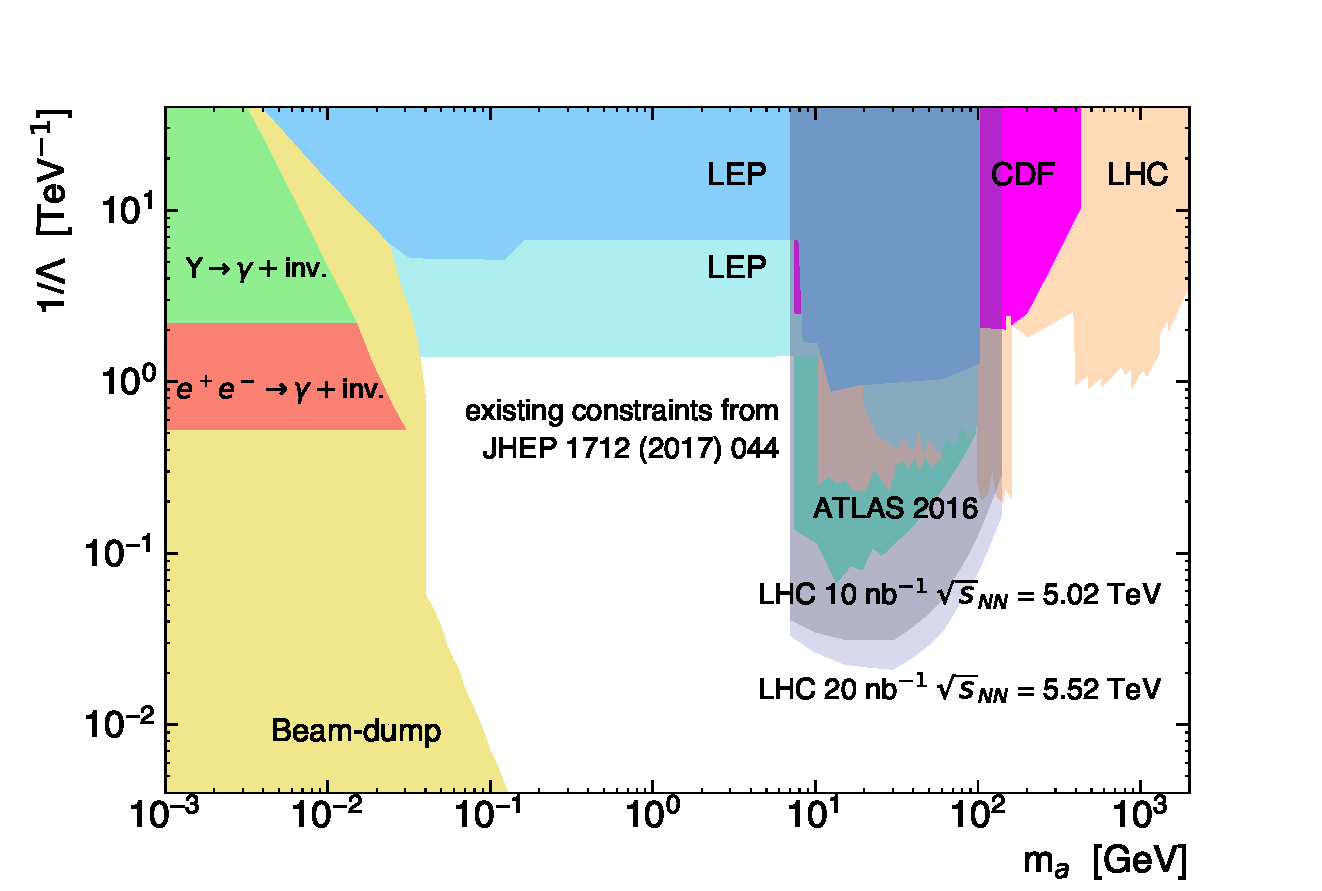
\includegraphics[scale=0.6]{\main/beyond/fig/ALPLimits_atlas_cms.pdf}
%  \caption{Compilation of exclusion limits obtained by different experiments (see text). ATLAS 2016 represents the exclusion limit derived from the recent LbyL cross section measured in Pb–-Pb collisions by ATLAS. In dark grey, LHC 10 nb −1 is shown corresponding to the analysis described in the text. Also in light grey, the LHC 20 nb −1 limit for s NN = 5.52 TeV is presented. A more complete version of the existing constraints on ALPs masses versus coupling, including the constraints in the sub meV range from astrophysical observations and from dedicated experiments such as CAST can be found in Ref.~\cite{Bauer:2017ris}.}
%  \label{fig:alp-lambda-limits}
%\end{figure}
%-------------------------------------------------------------------




\clearpage
%%%%%%%%%%%%%%%%%%%%%%%%%%%%%%%%%%%%%%%%%%%%%%%%%%%%%%%%%%%%%%%%%%%%%%
\subsection{Proton-oxygen collisions for cosmic ray research}
\label{sec:pOcosmic}
%%%%%%%%%%%%%%%%%%%%%%%%%%%%%%%%%%%%%%%%%%%%%%%%%%%%%%%%%%%%%%%%%%%%%%
{ \small
\noindent \textbf{Coordinators}: Hans Dembinski (MPI for Nuclear Physics, Heidelberg)

\noindent \textbf{Contributors}: 
T.~Pierog (Karlsruhe Institute of Technology), 
R.~Ulrich (Karlsruhe Institute of Technology)
}

\begin{figure}
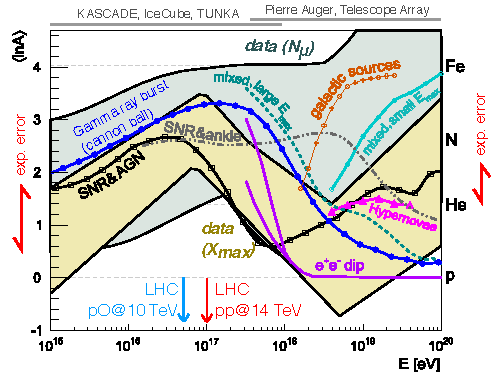
\includegraphics[width=0.5\textwidth,trim=5 -5 20 0]{\main/beyond/fig/lna_uncertainty.pdf}
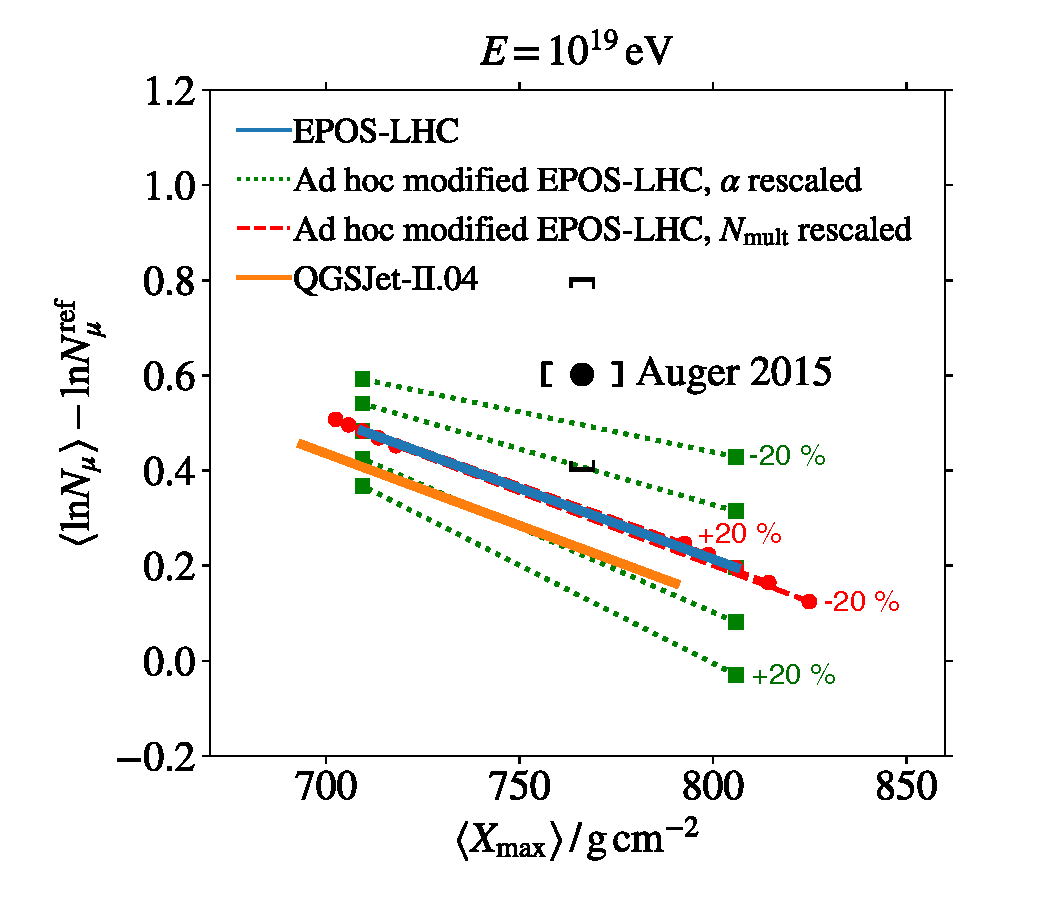
\includegraphics[width=0.5\textwidth,trim=-20 0 30 0]{\main/beyond/fig/epos_mod.pdf}
\caption{\emph{Left panel:} Mass composition of cosmic rays quantified by $\mlna$ as a function of cosmic ray energy $E$. See Ref.~\cite{kampert_cr_review} for references to data (bands) and model predictions (markers and lines), and the text for a discussion. \emph{Right panel:} Impact of changes of the hadron multiplicity $\nmult$ and the energy fraction $\alpha$ which goes into neutral pions in collisions at the LHC energy scale on EPOS-LHC predictions for $\xmax$ and $\lnnmu$ in $10^{19}$\,\si{eV} air showers, compared to Auger data~\cite{Aab:2014pza}. The model lines represent all values that can be obtained for any mixture of cosmic nuclei from proton (bottom right) to iron (top left). The dashed and dotted lines represent modifications of $\nmult$ and $\alpha$ in steps of $\pm$10\% from their nominal values.}
\label{fig:cosmic_rays}
\end{figure}

The recent coincident observations of gamma rays and neutrinos from the flaring blazar TXS 0506+056 confirmed that active galactic nuclei produce high-energy cosmic rays~\cite{IceCube:2018dnn}. This long awaited finding demonstrates that sources of cosmic rays are linked to the most violent places in our universe. Measurements of cosmic rays contribute to the understanding of the high-energy universe. Since cosmic rays are charged and bent by magnetic fields in space onto chaotic paths, their arrival directions are highly isotropic, but their mass composition contains a unique imprint of the source physics. Precision measurements of minimum-bias events in proton-oxygen collisions have the unique power to resolve current ambiguities in the mass composition.

Cosmic rays are nuclei from protons to iron (heavier elements are negligible). The energy-dependent mass composition of cosmic rays is characteristic for different source scenarios, as shown in Fig.~\ref{fig:cosmic_rays}, left-hand-side, which displays predictions (lines and markers) of the mean-logarithmic-mass $\mlna$ of cosmic rays. Above particle energies of $10^{15}$\,\si{eV}, $\mlna$ can only be indirectly inferred from extensive air showers, huge secondary particle cascades produced by collisions between cosmic rays and nuclei in the atmosphere. The two leading observables to infer $\mlna$ are the depth $\xmax$ of the shower maximum in the atmosphere (yellow band in Fig.~\ref{fig:cosmic_rays}), and the number $\nmu$ of muons produced in the shower (green band in Fig.~\ref{fig:cosmic_rays}). The width of those bands has two main contributions: the experimental uncertainties, and the model uncertainties inherent in converting the air shower observables into $\mlna$.

Leading experiments achieve an instrumental accuracy of 10\,\% of the proton-iron difference, which would strongly discriminate between source scenarios, but air shower simulations are required to convert $\nmu$ and $\xmax$ to $\mlna$ and this adds a large model uncertainty. The simulations use the multi-purpose heavy-ion event generator EPOS-LHC~\cite{Werner:2005jf}, or specialized hadronic interaction models such as \mbox{QGSJet-II.04}~\cite{Ostapchenko:2010vb} and SIBYLL-2.3c~\cite{Riehn:2017mfm}. All are designed to describe nucleus-nucleus and soft-QCD interactions by extrapolating combinations of Regge field theory tuned to available data and perturbative QCD. Uncertainties in these models arise from a lack of data on multiparticle production in the very forward phase-space in hadron-nucleus interactions at the TeV scale.

LHC measurements have already reduced the spread of model predictions for $\xmax$ in the latest generation of models. High-precision measurements of the inelastic cross-section (see e.g.~\cite{Aaij:2018okq} and references therein) had a large impact. Further measurements now have the potential to make the spread negligible. The model spread for $\nmu$ is still large and predictions are not consistent with $\xmax$ for cosmic rays with the same mass. There is overwhelming evidence from air shower experiments~\cite{Dembinski:2018UHECR,Aab:2014pza,Dembinski:2017zkb,Kokoulin:2009zz,Abbasi:2018fkz} that the muon number $\nmu$ is underestimated in simulations starting from $10^{17}$\,eV, corresponding to 14\,TeV cms energy accessible by the LHC. Shown in Fig.~\ref{fig:cosmic_rays}, right-hand-side, is a representative data point from the Pierre Auger Observatory, which is well above EPOS-LHC predictions. EPOS-LHC and SIBYLL-2.3c produce most muons of all models. This is called the \emph{Muon Puzzle}.
% The muon discrepancy casts a shadow on the general confidence in air shower simulations.

% The impact can be see in Fig.\ref{fig:cosmic_ray_related_lhc_measurements}, left-hand-side, which compares up-to-date models (solid lines) tuned to LHC data to predictions from older models (dashed and dotted lines).

% why we want to discuss ``forward'' in the context of ``pO''???
%The forward direction is in particular important for the air shower development, and naturally difficult to %instrument at accelerators. This results in relatively large model uncertainties due to missing constraints %by data in the relevant phase space.

Two aspects of multi-particle production with a strong effect on $\nmu$ have been identified\cite{Ulrich:2010rg}, the hadron multiplicity $\nmult$ and the energy fraction $\alpha$ that goes into neutral pions. The impact of changing these variables in EPOS-LHC at $13$\,TeV cms energy and extrapolating upward in energy is also shown in Fig.\ref{fig:cosmic_rays}, right-hand-side. A combined measurement to 5\,\% accuracy of both variables at the LHC would reduce the model uncertainty for the conversion of $\xmax$ to $\mlna$ well below the experimental uncertainty of 10\,\%, and has the clear potential to resolve the discrepancy in the muon number $N_\mu$. To reach the accuracy goal, the following measurements are desired:
\begin{itemize}
\item Double-differential production cross-section for charged pions, kaons, and protons: \\ ALICE $|\eta| < 0.9$, LHCb $2 < \eta < 5$
\item Production cross-section for neutral pions and neutrons: LHCf $8.4 < \eta$.
\item Energy flow over pseudo-rapidity, separated for hadrons and gammas:\\ CMS+CASTOR $-6.6 < \eta < 5.2$, ATLAS $-4.5 < \eta < 4.5$.
\end{itemize}
Energy flow measurements separated by hadronic and electromagnetic energy deposit constrain both $\nmult$ and $\alpha$, and can be done further forward than direct measurements of charged tracks.

\begin{figure}
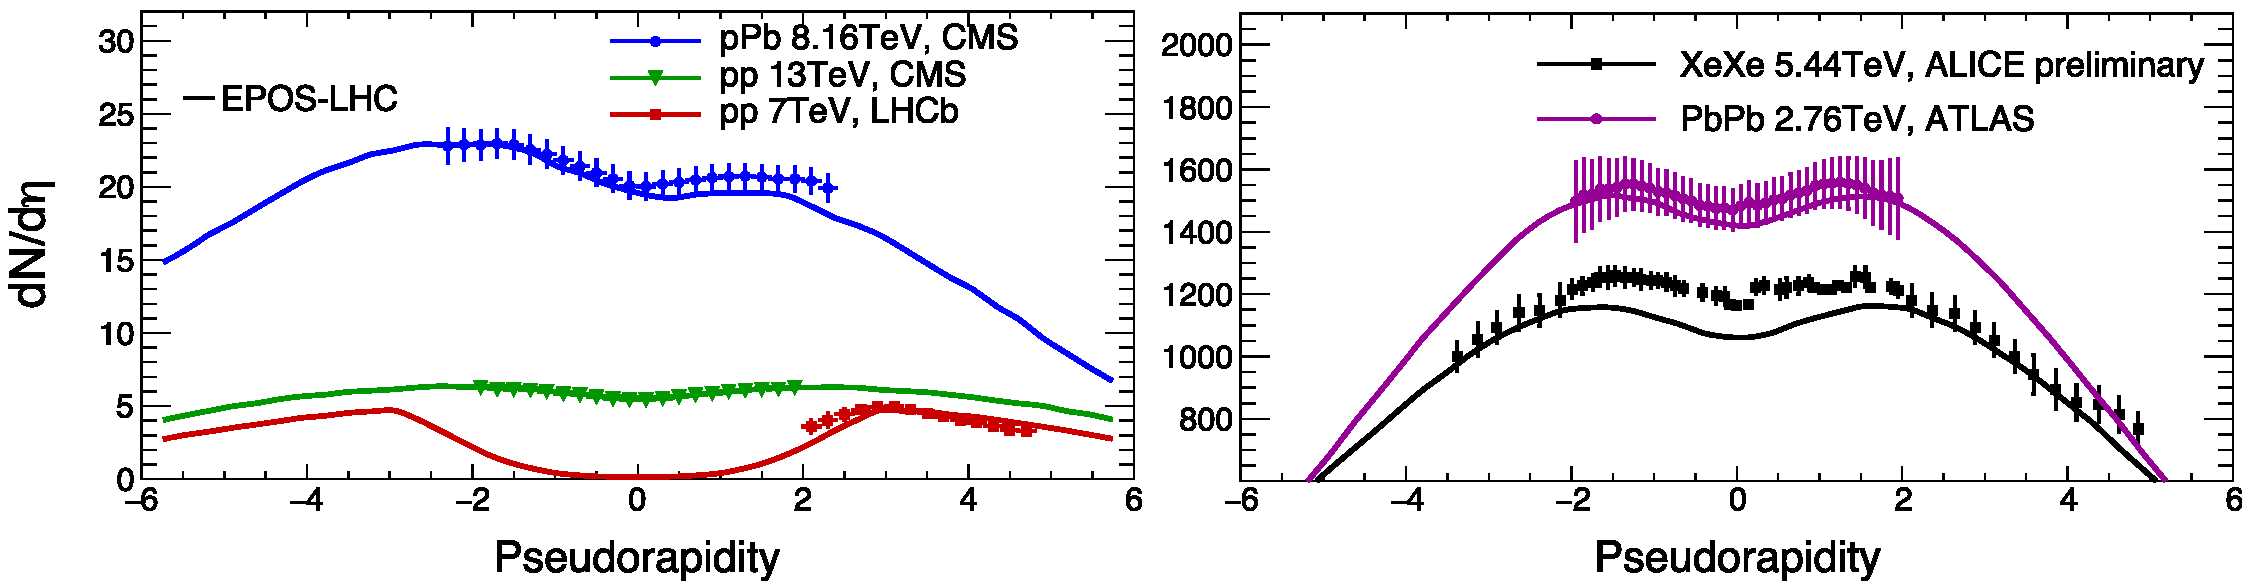
\includegraphics[width=\textwidth]{\main/beyond/fig/multiplicity_tuning_mod.pdf}
\caption{Comparison of charged particle multiplicity measurements at different center-of-mass energies and in different colliding systems with the EPOS-LHC model~\cite{Kim:2018ink}. Both plots show $\text{d} N/\text{d}\eta$.}
\label{fig:multiplicity_tuning}
\end{figure}

The impact projections assume that $\nmult$ and $\alpha$ are measured in proton-oxygen collisions at the LHC, which directly mimic interactions of cosmic rays with the atmosphere. Constraining $\alpha$ and $\nmult$ to 5\,\% with existing \pp and \pPb data is very challenging~\cite{dEnterria:2018kcz}, since forward-produced hadrons experience strong nuclear modification\cite{Aaij:2017cqq,Acharya:2018qsh,Adriani:2015iwv}. A sufficiently accurate theory to predict nuclear modification in the \pO system based on \pp and \pPb data is not yet available, and a simple interpolation is not realiable since both systems are far away in $\ln A$.
% Furthermore the collective effects which were not expected to be observed in light system (and as a consequence not implemented in specialized models for air shower simulation) seems to be very present in p-Pb~\cite{ALICE:2017jyt}.
The difficulty of predicting hadron production in ion collisions is demonstrated in Fig.~\ref{fig:multiplicity_tuning}. EPOS-LHC predictions for \XeXe collisions significantly underestimate the observed yields in the central region, despite a satisfactory description of \pp, \pPb, and \PbPb collisions. The deviations in \XeXe are much larger than what is expected from a simple interpolation~\cite{Kim:2018ink}. The dominant nuclear effects are expected to be different for light and heavy collision partners. Light nuclei are described by the shell model and nucleon correlations are important. Lead nuclei can be described by a simpler model, essentially a Wood-Saxon potential with reduced nucleon correlations that cannot be probed well in experiments.

Selecting peripheral \pPb collisions to mimic p-air collisions with the same number of binary collisions was considered as an alternative to direct \pO measurements, but it is not viable. Centrality in \pPb collisions is extracted from the data using various centrality estimators with different selection biases. These biases would increase the uncertainty of the proposed measurements well beyond the target of 5\,\%~\cite{Adam:2014qja}. However, \pO measurements could provide a sensitive test of centrality estimators since the thickness of the oxygen nucleus and hence the average number of wounded nucleons is about a factor of two smaller. The advantages of estimating centrality in a small ion system are discussed in Sect.~\ref{sect:smallsystems_OO}.

The luminosity requirements to reach the physics goals are moderate. A statistical accuracy better than 5\,\% can be achieved with a few 100\,M minimum-bias events, which can be accumulated within a day of data-taking. Luminosity calculations for light ion systems are given in Sect.\ \ref{sec:lightions}. The setup of \pO collisions would follow the successful rapid set-up procedure previously used in the 2012 \pPb run and the 2017 \XeXe run, as described in Sect.~\ref{sec:pOrun}.

It is worthwhile noting that a period of oxygen acceleration in the SPS would also provide the opportunity to complement cosmic-ray related measurements of nuclear fragmentation at NA61/SHINE\cite{Aduszkiewicz:2287004,Aduszkiewicz:2309890} at beam momenta of $150\,A\,\text{GeV}/c$. These measurements aim at improving our understanding of the cosmic-ray propagation in the Galaxy and to evaluate the cosmic-ray background for signatures of astrophysical dark matter~\cite{Genolini:2018ekk}. Another opportunity is the study of very forward production of hadrons in the \pO system at $\sqrtsnn \sim 100$ at the LHCb experiment, by colliding the oxygen beam with proton gas provided by an upgraded SMOG system, as described in Sect.~\ref{sec:fixedtarget}.

% This explicitly is not limited to just  the center-of-mass energy, but is very critical also for the ``forward'' phase space, and in particular for nuclear effects. The quality of the extrapolation can only be checked and improved with dedicated measurements. For example, in Fig.~\ref{fig:multiplicity_sqrt} the extraplation of central charged particle multiplicty is illustrated. The models EPOS-1.99, QGSJet01 and SIBYLL2.1 were all tuned up to Tevatron energies ($\sqrt{s}=900$\,GeV), and indicated good agreement with LHC data at $\sqrt{s}=2.36\,$TeV but performed very poorly on $\sqrt{s}=7\,$TeV LHC data. However, the LHC-tuned models EPOS-1.99, QGSJetII and SIBYLL2.3 do now a very good prediction at $\sqrt{s}=13$\,TeV, but start to diverge beyond that. It seems we can make reasonable model extrapolation of about a factor of two in energy.


% \begin{figure}
% \includegraphics[width=0.5\textwidth]{\main/beyond/fig/EnergyDependenceMultiplicity.pdf}
% \includegraphics[width=0.5\textwidth]{\main/beyond/fig/multiplicity_tuning.pdf}
% \caption{\emph{Left panel:} Comparison of charged particle multiplicity measurments at
% different center-of-mass enrergies and in different colliding systems.
% \emph{Right panel:} Dependence of the central ($|\eta|<0.5$) charged paticle
% multiplicity on center-of-mass energy.}
% \label{fig:cosmic_ray_related_lhc_measurements}
% \end{figure}

% For nuclear effects the impact of extrapolation has been even less clear, due to the lack of data. In cosmic ray physics the typical scenario are light nuclei collision.

%TODO: Talk about convergence in pp, but divergence in describing
%pO. Need to show another plot of hadron multiplicity and Eem/Ehad
%ratio with bands of current uncertainty.

% We might alternatively include a paragraph by Michael about the need of primary oxygen for NA61...


\clearpage
%%%%%%%%%%%%%%%%%%%%%%%%%%%%%%%%%%%%%%%%%%%%%%%%%%%%%%%%%%%%%%%%%%%%%%
\subsection{Fixed-target prospects with LHC beams}
\label{sec:fixedtarget}
%%%%%%%%%%%%%%%%%%%%%%%%%%%%%%%%%%%%%%%%%%%%%%%%%%%%%%%%%%%%%%%%%%%%%%
{ \small
\noindent \textbf{Contributors}: G. Graziani (INFN, Firenze), Frederic Fleuret (LLR/{\'E}cole Polytechnique), C. Hadjidakis (IPNO, Paris), E. Maurice (LLR/{\'E}cole Polytechnique),  Luciano Pappalardo (University of Ferrara), Patrick Robbe (LAL, Paris),  L. Massacrier (IPNO, Paris),  Pasquale Di Nezza (INFN, Frascati), B. Trzeciak (Institute for Subatomic Physics, Utrecht)
}

The physics opportunities offered by a fixed-target programme at the LHC have been developped in several publications of the AFTER@LHC study group \cite{Brodsky:2012vg, Lansberg:Adv2015} and can be summarised as follows:
\begin{itemize}
\item advance our understanding of the large-$x$ gluon, sea quark and heavy-quark content in the nucleon and nucleus;
\item advance our understanding of the dynamics and spin of gluons inside polarised nucleons (if a polarised target were used);
\item advance our understanding of the properties of the Quark-Gluon Plasma formed in heavy-ion collisions between the SPS and the largest RHIC centre-of-mass energies.
\end{itemize}
The LHCb Collaboration has already started a fixed-target physics programme using both proton~\cite{Aaij:2018svt,Aaij:2018ogq} and Pb beams colliding with noble-gas nuclei at rest injected with the SMOG system~\cite{SMOG}: the future plans for the LHCb fixed-target programme are discussed in Section~\ref{sec:FTLHCb}. Studies are ongoing within the ALICE Collaboration to explore the complementary physics potential with the ALICE detector and the implementation options (Section~\ref{sec:FTALICE}). 

\subsubsection{Status and future plans in LHCb}
\label{sec:FTLHCb}


The LHCb experiment has pioneered fixed target physics at the LHC since Run 2, 
using noble-gas targets (helium, neon and argon) obtained by injecting the gas directly in 
the LHC vacuum pipe in the proximity of the LHCb~collision point
through the SMOG device~\cite{smog}.
The nominal target gas pressure of $2 \times 10^{-7}$ mbar corresponds,
for a typical LHC beam of $10^{14}$ protons, to a luminosity of 
$6 \times 10^{29} \text{cm}^{-2}\text{s}^{-1}$ for collisions occurring in one
meter of gas along the beam direction, which is roughly the acceptance of the
LHCb vertex detector.

The forward geometry of the detector is particularly well suited for
this configuration.  It provides three units
of pseudorapidity corresponding to mid and backward rapidities ($-2.8 < y_{cms}< 0.2$
for a beam energy of 6.5 TeV), fully equipped with tracking and particle identification. 
Proton-nucleus and Pb-nucleus collisions using fixed targets of different
nuclear size can be studied at the energy scale of $\sqrtsnn \sim 100$
GeV with unique coverage of the high-$x$ regime in the target nucleon.

The samples collected during Run 2, corresponding
to integrated luminosities up to about $100~\invnb$, 
allowed to perform 
studies of particle production which are of particular relevance
to cosmic ray physics~\cite{LHCb-PAPER-2018-031}, and to
collect unprecedented samples of charmed hadrons in
fixed-target collisions at this energy
scale~\cite{LHCb-PAPER-2018-023}. 
These data can provide unique inputs to
discriminate cold nuclear matter effects in heavy-flavour production
from the effect of deconfinement, and to study nuclear PDFs 
at large $x$. The physics reach of heavy-flavour studies is presently
limited by the size of these samples. Measurements of absolute
cross-sections are also limited in accuracy by the determination of the
luminosity, since the gas pressure can be controlled only
within $\pm 50\%$ with the SMOG device. For the first fixed-target physics
results, the integrated luminosity has been determined from the rate of
elastically scattered atomic electrons with a precision of
6\%~\cite{LHCb-PAPER-2018-031}. 

An upgraded gas target device, named SMOG2, is currently being developed, and expected
to be operational already during Run 3. 
In the new setup, the gas is contained in a storage cell, consisting
of a 20-cm-long open-ended tube with a diameter of 1 cm, feeded by a capillary.
It allows to increase the gas density in the target
by at least one order of magnitude with respect to SMOG, reaching
luminosities of order $10^{31}~\text{cm}^{-2}\text{s}^{-1}$ with
proton beams.
The target is placed upstream, from -50 to -30 cm, the nominal  LHCb
collision point and is thus not overlapping the luminous pp region.
This opens the possibility to acquire fixed target events
simultaneously with collision events with negligible impact to the
pp physics program.
The new setup would also allow other gases to be injected, notably hydrogen and deuterium, providing
pp collisions in fixed-target mode as a reference for all pA
collision samples, and extending the physics case to the study
of the three-dimensional structure functions of the nucleon through
spin-independent observables~\cite{3dpdf}. Heavy noble gases as Kr
and Xe would also be usable.
The device will be equipped with a gas feed system, allowing
to know the target gas density at 1\% level.

Assuming that about 10\% of the beam intensity can be exploited for
fixed-target physics, either in synergy with $pp$ data taking or through dedicated runs,
samples corresponding to integrated luminosities of order $0.1~\textrm{fb}^{-1}$
(using proton beams) and $0.1~\textrm{pb}^{-1}$ (using Pb beams) 
can be collected per year, also profiting from the increased beam
intensity provided by the HL-LHC.

Samples of this size would allow copious production of Drell-Yan
and heavy flavour states, including $\textrm{b}\overline{\textrm{b}}$ mesons.
As an example, rough estimates are provided in
Table~\ref{tab:ftyields} for the yields of reconstructed events in an assumed sample of pAr collisions corresponding to $0.1~\textrm{fb}^{-1}$.
Substantial advancements in the understanding of parton
distributions for gluons, antiquark and heavy-quarks 
at large $x$, where PDFs are now poorly constrained, are
foreseeable~\cite{after,Hadjidakis:2018ifr}. The precise determination
of heavy hadron production at large $x$ is expected to clarify
the  extent of the intrinsic heavy quark content
in the nucleon~\cite{Brodsky:1980pb,Brodsky:2015fna}, and to constrain
modifications of the nuclear PDFs due to initial state effects
(anti-shadowing and EMC effect~\cite{Geesaman:1995yd}, saturation
effects~\cite{Albacete:2014fwa}).
Sequential quarkonia suppression is a main signature for
deconfinement~\cite{Matsui:1986dk}, but is also affected by final
state effects as break-up of the heavy quark  pair~\cite{Vogt:2001ky}
and statistical recombination~\cite{BraunMunzinger:2000px}.
The rich samples of  different quarkonia states reconstructed 
in fixed target data will allow to
investigate sequential suppression at an energy scale
between the SPS and RHIC/LHC, for 
collision systems ranging from pp to PbXe.
The study of collisions of Pb beams on heavy nuclei has been 
limited in Run 2  by the detector tracking capabilities and would
greatly profit from the higher detector granularity offered by the 
LHCb upgrade 1 and upgrade 2 detectors.


\begin{table}[tb]
\caption{Expected yields of reconstructed events for some benchmark channels
using the largest fixed-target data sample acquired with SMOG during
the LHC Run 2, and possible with SMOG2, using as example a $p$Ar sample of $0.1~\textrm{fb}^{-1}$.
}
\label{tab:ftyields}
  \centering
  \begin{tabular}{lcc}
                               & SMOG                   &   SMOG2     \\
                               &  ~~largest sample~~    &    example  \\
                               &  $p$Ne@68 GeV            &  ~~$p$Ar@115 GeV~~   \\ \hline
Integrated luminosity          & $\sim$ 100 $~\textrm{nb}^{-1}$      &    100 $\textrm{pb}^{-1}$  \\
syst. error on J/$\psi$ x-sec.    &     6 - 7\%            &    2 - 3  \%     \\
J/$\psi$ yield                    &      15k               &      35M          \\
D$^0$ yield                      &      100k              &      350M         \\
$\Lambda_c$ yield                      &       1k               &      3.5M         \\
$\psi$(2S) yield                 &       150              &      400k         \\
$\Upsilon$(1S)~ yield                   &       10               &       13k         \\
Low-mass ($5<M_{\mu\mu}<9~\textrm{GeV}/c^{2}$) Drell-Yan yield       &       10               &       20k         \\
  \end{tabular}
\end{table}


The fixed-target program also presents a very good testbed for the
hydrodynamic description of the QCD medium produced in heavy-ion collisions
down to the energy of $\sqrtsnn \sim 100$~GeV, thanks to the
considerable pseudorapidity coverage, with particle identification capability for pions,
kaons and protons as well as neutral particles $\phi$, $K^0_S$ and $\Lambda^0$.
Measurements of flow observables and correlations can contribute in particular to shed light on the
extension of the hydrodynamic description~\cite{Song:2007ux,Schenke:2010rr} 
successful at top RHIC energy and at the LHC towards lower beam
energies requiring an appropriate 
treatment of baryon density~\cite{Karpenko:2015xea}, and a fully 3 dimensional initial state~\cite{Shen:2017bsr}.
This can provide important inputs to the search for the critical point in
the QCD phase diagram~\cite{Stephanov:2004wx,Luo:2017faz}. 
In addition, the extension of the fluid dynamical paradigm towards smaller collision systems as an
explanation of the experimental findings in proton(deuteron)-nucleus and \pp~collisions
at the LHC~\cite{Khachatryan:2010gv,CMS:2012qk,Abelev:2012ola,Aad:2012gla,Aaij:2015qcq} and
at RHIC~\cite{Adare:2018toe} can be probed in a novel kinematic regime.


The study of ultra-peripheral collisions in the fixed target
configuration also offers a complementary kinematic regime to
the similar studies in beam-beam collisions discussed in
Section\ref{10}. 
An intriguing possibility would be the observation of $\eta_c$ photoproduction in the PbAr sample, where the cross
section is estimated to be of order $1$~nb~\cite{Goncalves:2015hra}. This would constitute 
a confirmation for the existence of the odderon, since the $\eta_c$ state can't be produced in the $\gamma$-pomeron 
process and would be under threshold for the $\gamma$-$\gamma$ process in fixed-target PbA collisions.
Large samples of exclusively produced $\rho^0$ and $\omega$ are also expected~\cite{Goncalves:2018htp}.


Studies of proton collisions on light nuclei provide crucial inputs to the
understanding of cosmic ray propagation in the interstellar medium
(using H and He targets) and in the atmosphere (using N and O
targets). The interpretation of the precise measurements of the
antiproton component in cosmic rays, performed in the last decade by the
PAMELA~\cite{Pamela} and AMS-02~\cite{AMS02} space-based missions, is
presently limited by the knowledge of the antiproton production
in the interstellar medium. The first measurement of antiproton production
in $p$He collisions has been performed by LHCb with Run 2
data~\cite{LHCb-PAPER-2018-031} and has been used to improve the 
sensitivity to a possible dark matter contribution to the cosmic antiproton
flux~\cite{Reinert:2017aga,Korsmeier:2018gcy}. 
During Run 3, it is planned to extend these studies with a hydrogen
target. The production of antineutrons can also be inferred indirectly
by evaluating isospin violation in antiproton production 
from proton-hydrogen and proton-deuterium collisions.

A better understanding of the bulk of particle production in
high-energy hadronic collisions is also crucial to the modeling of
atmospheric showers induced by ultra-high-energy cosmic rays. 
Despite the moderate energy scale, fixed target data offer the
unique possibility to use a wide range of nuclear targets, including
nitrogen and oxygen, and to study production at large $x$. 
The main background for the observation of the astrophysical
high-energy neutrino flux, recently established by 
the IceCube collaboration~\cite{Aartsen:2013jdh}, originates from
neutrinos of PeV energy produced from decays of charmed hadrons in
atmospheric showers. A relevant uncertainty on this background
is related to the possible intrisic charm contribution to the charm
PDF at large $x$~\cite{Laha:2016dri}.  
Knowledge of light hadron production, notably baryons, at large $x$ will allow 
to improve the modeling of the number of muons produced in the lateral
development of the showers, which is a key observables to infer the
mass composition of ultra-high-energy cosmic rays, as discussed in Section~\ref{11.3}.


More ambitious projects for future target upgrades have also been proposed for a possible installation
in LHCb on the time scale of HL-LHC. These are beyond the baseline
LHCb Upgrade 2. A polarised gas target similar to that used in
HERMES~\cite{Airapetian:2004yf}, installed upstream of the LHCb vertex
detector, would make LHCb a key contributor to spin physics. 
With this option, LHCb would have access to single spin asymmetries in an
unique kinematic range for a variety of final states, including unique
measurements with quarkonium and Drell-Yan lepton
pairs~\cite{Kikola:2017hnp}. 
Measurements of the three-dimensional structure of nucleons from hadron collisions would be highly
complementary to the program at the electron-ion collider, which is proposed on a
comparable time scale.


\subsubsection{Opportunities with ALICE}
\label{sec:FTALICE}


One of the main strengths of ALICE in fixed target mode would be its large rapidity coverage. Assuming a target location at $z=0$, the ALICE muon spectrometer (and future Muon Forward Tracker) would access the mid- to backward rapidity in the centre-of-mass frame ($-2.3 < y_{\rm cms} < -0.8$)\footnote{\label{note1} considering an incident proton beam on the target. For an incident lead beam, the muon spectrometer rapidity coverage is $-1.8 < y_{\rm cms} < -0.3$ and central barrel coverage $-5.2 < y_{\rm cms} < -3.4$}. In addition, the long absorber in front of the muon tracking station is an asset for background rejection and Drell-Yan studies at low energy. The ALICE central barrel offers a complementary coverage to the muon arm by accessing the very backward rapidity region ($-5.7  < y_{\rm cms} < -3.9$), reaching the end of phase space for several probes. Thanks to its excellent particle identification capabilities, particle detection and identification down to low $p_{\rm T}$, unique measurement of soft probes and open heavy flavours can be pursued. Another asset of the ALICE apparatus is the capability to operate with good performances in a high particle density environment. Access to most central AA collisions at $\sqrt{s_{\rm NN}}$~=~72~GeV should be possible if the interaction rate remains low. In addition, the ALICE Collaboration could potentially devote a significant data taking time to a fixed-target programme (especially with the proton beam), allowing the collection of large integrated luminosities and the investigation of several target species. Two main solutions are being investigated to deliver fixed target collisions to ALICE: an internal gaseous target or an internal solid target (coupled to a bent crystal to deflect the beam halo). On the one hand, a gas-jet or a storage cell (with levelled gas pressure) would allow to deliver about 45 pb$^{-1}$ of proton-polarised hydrogen collisions to ALICE per year (260 pb$^{-1}$  in case of proton-unpolarised H$_{2}$ collisions), and 8 nb$^{-1}$ of Pb-Xe collisions. With such system the target can be polarised, but requires large space to be installed (most likely outside the ALICE barrel magnet), requiring thus the need of additional detectors for vertexing and additional studies of the tracking performances of the TPC in such conditions. A simple unpolarised storage cell might potentially be used closer to the current ALICE IP. On the other hand, the usage of an internal solid target coupled to a bent crystal has the advantage of more portability, allowing one to install the target closer to the nominal ALICE IP and thus benefiting of the optimal performances of the current ALICE apparatus. With such a device 37 pb$^{-1}$ (6 pb$^{-1}$) of p-C (p-W) collisions, and 5 nb$^{-1}$ (3 nb$^{-1}$) of Pb-C (Pb-W) collisions could be registered in ALICE per year. The performances for several key probes have been investigated in simulations and some physics perspectives are highlighted below. 
\begin{itemize}
\item{Quarkonia : Very large yields are expected for charmonia ($\sim 10^{6}$) in the ALICE muon spectrometer both in pp and Pb-Xe collisions considering one LHC year of data taking. The $\Upsilon$(1S) will also be within reach. Looking at quarkonium suppression as a function of rapidity and the system size would allow one to search for the QGP phase transition, and provide a measurement of the medium temperature for centre-of-mass energies between the ones probed at RHIC and the SPS. In pA collisons, $\Upsilon$(1S) could be used to probe large $x$ in the target, in order to constrain gluon anti-shadowing and EMC effect.}
\item{Drell-Yan : A precise measurement of the Drell-Yan process with the muon spectrometer can probe initial state effects on quarks from pA to AA collisions. The correlated background from $b\overline{b}$ and $c\overline{c}$ pairs in the dimuon decay channel is largely reduced at the lower center-of-mass energy of the fixed target mode, with respect to the TeV energy range.}
\item{Open Heavy Flavours : At $y_{\rm lab} \sim$ 1 about 500 (100) D$^{0}$ are expected to be produced per 0.1 rapidity unit per year in pp (Pb-W) collisions, respectively. The ALICE central barrel is probing the end of the D meson phase space, at very large-$x$, where the contribution of the intrinsic charm component in the proton could largely increase the D meson yield. Hence the ALICE central barrel is well suited to study the large-$x$ intrinsic charm component in the proton.}
\item{Identified charged particles : In few hours of Pb-Pb data taking, it would be already possible to collect 10$^{6}$ minimum bias events with the ALICE central barrel and reach an absolute statistical uncertainty of 0.01 on the elliptic flow coefficient $v_{2}$ for pions and protons, 0.02 for kaons, and 0.05 for antiprotons in semi-central events. Particle yields and flow coefficients measured at large rapidities are powerful tools to access the medium shear viscosity and temperature. High precision complementary studies to the ones performed at RHIC would clarify the collectivity picture between SPS and LHC results. In addition, measurement of identified particles up to very large rapidities would complement the limiting fragmentation studies carried out by the BRAHMS and PHOBOS experiments at RHIC.} 
\item{Strangeness : Thanks to the large yields ($\sim$10$^{8}$ per 0.1 rapidity unit per year) of $\Lambda$ expected to be produced in the ALICE central barrel in proton-polarised proton collisions, a precise measurement of the longitudinal spin transfer D$_{LL}$ of the $\Lambda$ hyperon could be carried out. This would allow one to constrain the spin-dependent strange quark (antiquark) densities at large negative $x_{F}$.}
\end{itemize}

Studies are ongoing on other key observables, such as antiproton measurements in the central barrel as a key input for cosmic ray physics, photoproduced J/$\psi$ single transverse spin asymmetry measurements in the muon spectrometer to constrain the gluon GPDs and the search for the photoproduction of hidden charm pentaquark states in the central barrel.



\end{document}
